\documentclass[12pt]{report}
\usepackage{graphicx} % Required for inserting images
\usepackage[spanish]{babel}


\usepackage{amsthm}  % Para los entornos de teoremas

\usepackage{pgfplots}
\pgfplotsset{compat=1.18}
\usepackage{amsmath, amssymb} % Para símbolos matemáticos
\usepackage{multicol}
\usepackage{caption}
\usepackage[a4paper, margin=2.5cm]{geometry} % Márgenes de 2.5 cm
\usepackage{hyperref}
\usepackage{float}
\usetikzlibrary{arrows.meta, positioning}
% Definición de entornos
\newtheorem{theorem}{Teorema}[section]  % Enumera los teoremas por sección
\newtheorem{lemma}[theorem]{Lema}       % Usa la misma numeración de los teoremas
\newtheorem{proposition}[theorem]{Proposición}
\newtheorem{corollary}[theorem]{Corolario}

% Definición con estilo diferente
\theoremstyle{definition}
\newtheorem{definition}[theorem]{Definición}
\newtheorem{example}[theorem]{Ejemplo}
\newtheorem{objetivo}[theorem]{Objetivo}

% Observaciones con estilo de remark
\theoremstyle{remark}
\newtheorem{remark}[theorem]{Observación}
\providecommand{\norm}[1]{\lVert#1\rVert}



\title{RESUMEN Aprendizaje Automático No Supervisado}
\author{Jose Carlos Martínez Bastida
\\ \small Notas hechas a partir del temario de AANS de UNIR}
\date{\today}

\begin{document}

\maketitle
\tableofcontents
\newpage

\chapter{Aprendizaje automático no supervisado}

\section{Definición de Aprendizaje no supervisado y ámbitos de uso}

El aprendizaje automático no supervisado se denomina así porque no hay un supervisor externo proporcionando retroalimentación sobre cómo debe ser clasificado un dato. Se parte de la premisa de que incluso sin el supervisor externo, se puede extraer conocimiento a partir de los datos sin procesar mediante la detección de patrones y estructuras de datos sin etiquetas.

Hay distintas áreas dentro del aprendizaje no supervisado o en las que diferentes técnicas de aprendizaje no supervisado se utilizan:

\begin{itemize}
    \item \textbf{Clustering} o agrupamiento: se busca reunir instancias similares dentro de los clústeres o grupos.

    \item \textbf{Reducción de la dimensionalidad}: se busca simplificar la complejidad de los datos mediante técnicas que permites explicar la varianza del conjunto de datos con menos dimensiones, lo que los hace más manejables. Técnicas como PCA son muy utilizadas también para la reducción de imágenes con una muy alta dimensionalidad.

    \item \textbf{Detección de anomalías}: se trata de encontrar patrones u observaciones inusuales o atípicos.

    \item \textbf{Procesamiento del lenguaje natural (PLN)}: se han utilizado técnicas como Latent Dirichlet Allocation (LDA) para descubrir temas dentro de un gran conjunto de documentos o textos. Esto permite, por ejemplo, la organización de bibliotecas.

    \item \textbf{Aprendizaje por refuerzo (RL)}: se basa en la interacción de un agente con su entorno para maximizar una recompensa acumulativa.
\end{itemize}


\section{Términos clave}

A continuación, se presentan una lista de términos clave para entender esta asignatura:

\begin{itemize}
    \item \textbf{Característica}: aquí nos referimos a una dimensión en el conjunto de datos. 

    \item \textbf{Clúster} o grupo: grupo de datos que comparten características similares.

    \item \textbf{Dimensionalidad}: número de características de un conjunto de datos.

    \item \textbf{Métrica de distancia}: medida que indica qué tan similares son dos puntos. Las métricas más comunes son la euclidiana, la Manhattan y la del coseno.

    \item \textbf{Outliers} o datos atípicos: puntos que se desvían del resto del conjunto de puntos. 

    \item \textbf{Centroide}: centro de un conjunto de datos.

    \item \textbf{Vectores y valores propios (eigenvectors y eigenvalues)}: términos de álgebra lineal que representan la dirección de la máxima variación en los datos y son utilizados para pasar de un espacio de alta dimensionalidad a un espacio de características menor.

    \item \textbf{Overfitting} o sobreajuste: término que se utiliza para decir que un modelo se ajusta muy bien con los datos de entrenamiento, pero es capaz de generalizar con datos no vistos anteriormente.

    \item \textbf{Hiperparámetros}: parámetros que se establecen en el momento inicial del entrenamiento.
\end{itemize}

\section{Retos en el aprendizaje no supervisado}
Algunos de los retos del aprendizaje no supervisado son:

\begin{itemize}
    \item \textbf{Determinar el número óptimo de clústeres en un dataset}: existen técnicas como la del codo, análisis de la silueta y el índice Davies-Bouldin para solventar este problema, pero al no saber, \textit{a priori}, el número de grupos en un dataset, siempre se necesitará de la experiencia humana para determinarlos.

    \item \textbf{Maldición de la dimensionalidad}: en un conjunto de datos con alta dimensionalidad, es posible no encontrar grupos con características comunes. Por ello, se tiende a reducir la dimensionalidad, pero siempre intentando preservar la estructura de los datos.

    \item \textbf{Escalabilidad de los algoritmos existentes}: cada vez hay una mayor cantidad de datos y los algoritmos de aprendizaje no supervisado pueden no ser óptimos en términos computacionales y predictivos.

    \item \textbf{Delimitar el ruido y los outliers}: los datos ruidosos pueden distorsionar la verdadera estructura de los datos. Los métodos de \textit{clustering} y filtro de ruido son elementales.

    \item \textbf{Interpretabilidad de los resultados}: se puede caer en interpretaciones subjetivas de los resultados al no tener categorías que asignen un significado objetivo. 

    \item \textbf{Métricas de éxito débiles}: las métricas sirven para validar el éxito o fracaso de los modelos. Se necesitan métricas definidas y robustas para medir la calidad y el desempeño de un modelo.
\end{itemize}


\section{Flujo de trabajo en el ANS}

Los pasos en un proyecto de aprendizaje no supervisado son los siguientes:

\begin{enumerate}
    \item Recolección de datos.

    \item Limpieza y preprocesamiento de datos. Aquí entra la eliminación de duplicados, el manejo de datos faltantes y el escalado de características (normalización, estandarización, escalado min-max...).
    Se incluye la codificación de variables categóricas y la transformación de datos, donde se aplican funciones sobre las características para estabilizar la varianza, y también técnicas de reducción de la dimensionalidad.

    \item Preparación de los datos.

    \item Elección y aplicación de un algoritmo no supervisado.

    \item Entrenamiento y parametrización del modelo.

    \item Interpretación de los resultados.

    \item Evaluación de los resultados.
\end{enumerate}


\subsection{Técnicas de transformación de datos}
Con el objetivo de reducir la asimetría y mejorar la predicción de los modelos,  se pueden aplicar técnicas lineales o no lineales sobre un conjunto de características.

Por ejemplo, si observamos que una característica parece seguir una distribución exponencial, se puede aplicar una transformación logarítmica (transformación lineal positiva).

Otra transformación ampliamente utilizada es la extensión de la logarítmica: la transformación de Box-Cox.

\begin{equation}
    y(\lambda) = \begin{cases} \frac{y^\lambda - 1}{\lambda}, & \text{if } \lambda \neq 0 \\ \ln(y), & \text{if } \lambda = 0 \end{cases}
\end{equation}


\begin{figure}[ht]
    \centering
    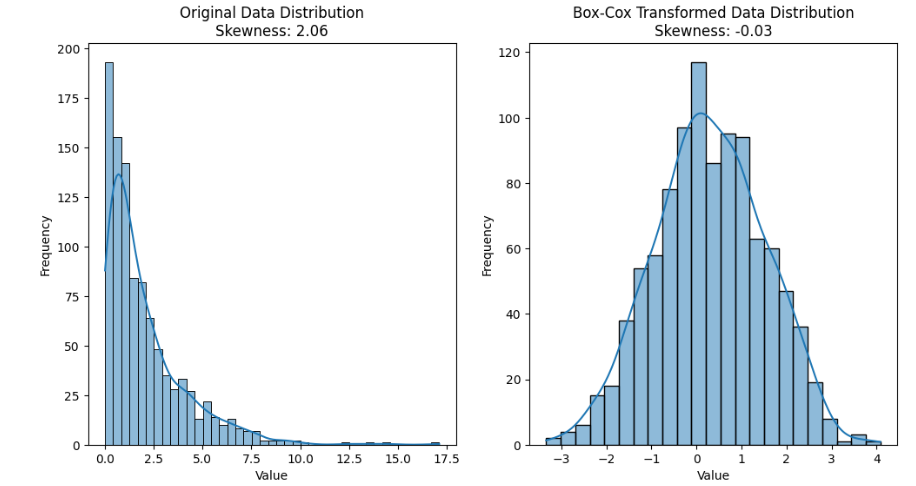
\includegraphics[width=0.75\linewidth]{imagenes/box-cox.png}
    \label{fig:box-cox}
\end{figure}

\subsection{Técnicas de discretización de datos}
Las técnicas de discretización convierten variables continuas en variables discretas, permitiendo ver los datos desde una perspectiva diferente. Este enfoque divide en rangos las variables continúas generando intervalos que tienen una etiqueta. De esta forma, el valor numérico pasa a una categoría o \textit{bins}.

Para el proceso de discretización, se pueden emplear árboles de decisión, para los que se aprovecha la \textbf{ganancia de información} como medida para delimitar los valores óptimos.

Otra técnica es el uso de cuantiles: dividir los valores continuos en cuatro cuantiles, donde cada cuantil encapsula una proporción igual de puntos de datos. 

\subsection{Técnicas de codificación de datos categóricos}
Los algoritmos de aprendizaje automático utilizan números y, por tanto, se hace necesario convertir los datos textuales a formato numérico.

La codificación es el proceso de convertir datos categóricos o textuales a numéricos, de modo que puedan usarse como entrada para que los procesen los algoritmos. Así, se permite que el modelo identifique patrones y haga predicciones basadas en esos patrones; esto ayuda a evitar sesgos al garantizar que todas las características tengan el mismo peso.

La elección del método de codificación puede tener un impacto significativo en el rendimiento del modelo, por lo que es importantes elegir una técnica adecuada según la naturaleza de los datos y los requisitos del modelo.

\begin{itemize}
    \item \textbf{Codificación One-Hot}: Una columna binaria se crea por cada categoría de la variable. Si la variable está presente se le asigna el valor de 1, si no se le asigna 0.

    \item \textbf{Codificación ordinal}: A cada categoría única se le asigna un valor entero único. Es más simple que la técnica anterior, pero tiene el inconveniente de que el algoritmo puede malinterpretar los números enteros asignados como si tuvieran una relación ordenada cuando no es el caso.

    \item \textbf{Codificación binaria}:  Las categorías se representan como dígitos binarios. Por ejemplo, si una variable tiene cuatro categorías  'Bueno',  'Malo',  'Regular'  y  'Excelente', se pueden representar como  0001, 0010, 0100 y 1000, respectivamente.

    \item \textbf{Codificación target}: Se utiliza con variables categóricas de alta cardinalidad; es decir, características con  muchas categorías únicas. Se calcula el valor objetivo promedio para cada categoría  y este valor promedio es utilizado para reemplazar la característica categórica.  Aunque toca utilizarla con precaución porque puede conducir a un sobreajuste.
\end{itemize}

\chapter{K-Means y sus fundamentos}
Los clústeres son la piedra angular del aprendizaje no supervisado. Entre los diferentes algoritmos de agrupación en clústeres, tenemos K-Means.

\section{K-Means}

El algoritmos K-Means particiona los datos en K clústeres distintos, cada uno de ellos representado por la media de los puntos. El objetivo es minimizar la varianza ínter-clúster, haciendo que los grupos tengan datos lo más diferentes posibles entre sí y, al mismo tiempo, asegurar que los elementos dentro de cada grupo sean lo más similares posible entre sí.

\subsection{Diagramas de Voronoi}

Los \textbf{diagramas de Voronoi} o \textbf{polígonos de Thiessen} son una forma de dividir el espacio en regiones basadas en la proximidad a un conjunto específico de puntos. Cada región en el diagrama de Voronoi está asociado a uno de estos sitios y contiene todos los puntos del espacio que están mas cerca de ese sitio que de cualquier otro.

En ciencia de datos, estos diagramas se utilizan para ilustrar cómo se agrupan los datos en torno a los centroides; en K-Means, cada región de Voronoi se corresponde a un clúster generado por el algoritmo.

Las características clave son:

\begin{itemize}
    \item Cada región está delimitada por las líneas bisectrices.

    \item Los vértices de los polígonos de Voronoi están ubicados en puntos donde tres o más sitios se encuentran equidistantes.

    \item Pueden ser bidimensionales o tridimensionales.
\end{itemize}


\subsection{El algoritmo K-Means: Paso a paso}

\begin{enumerate}
    \item Preprocesamiento de los datos: para mejorar la calidad y precisión de los modelos.

    \item Inicialización de centroides: se comienza el ciclo seleccionando aleatoriamente K puntos como centroides iniciales; los centroides son puntos que representan el centro de cada uno de los K grupos que se quieren identificar.

    \item Asignación de puntos a centroides: para cada punto del dataset, se calcula la distancia entre ese punto y cada uno de los centroides; luego, se asigna el punto al centroide más cercano.

    \item Actualización de los centroides: después de asignar cada punto a un centroide, se recalcula la posición de cada centroide como el centroide del grupo de puntos asignados a él: el nuevo centroide es el promedio de todas las coordenadas de los puntos asignados al grupo.

    \item Repetición: los dos pasos anteriores se repiten iterativamente hasta que los centroides dejen de cambiar de manera significativa o hasta que se alcance un número máximo de iteraciones.

    \item Convergencia: cuando los centroides permanecen constantes entre iteraciones y los puntos están asignados a los grupos de manera estable, hemos llegado a una situación de convergencia.

    \item Resultado final: tenemos un conjunto de K grupos, donde cada grupo está representado por su centroide.
\end{enumerate}


\section{Elección del número de clústeres}
Uno de los principales desafíos de los problemas de agrupamiento reside en elegir el número de grupos que representan al conjunto de datos. 

Un número de grupos erróneo implica que se tendrán grupos que no representan al conjunto de datos. Si conocemos el dominio de los datos, la tarea es más sencilla, pero no siempre es el caso.

Los dos principios básicos para encontrar el número óptimo de clústeres son:

\begin{itemize}
    \item Los puntos dentro del grupo deben ser lo más similares posible.

    \item Los puntos que pertenecen a distintos grupos deben ser lo más distintos posible.
\end{itemize}

Con esto en mente, vemos dos métricas que se utilizarán para hallar el número ideal de clústeres.

\subsection{Métricas}
\subsubsection{Inercia}

\begin{definition}
    La \textbf{inercia} se calcula como la suma de las distancias al cuadrado entre los puntos de datos y los centros de los grupos a los qu pertenece:

    \begin{equation}
        I=\sum_{i=1}^n\norm{x_i-\mu_{c(i)}}^2,
    \end{equation}

    donde: $n$ es el número total de puntos, $x_i$ es el i-ésimo punto de datos, $\mu_{c(i)}$ es el centroide del clúster al que pertenece el punto $x_i$ y $\norm{x_i-\mu_{c(i)}}^2$ es la distancia euclidiana entre el punto $x_i$ y su centroide correspondiente $\mu_{c(i)}$.
\end{definition}

\subsubsection{El método del codo}
\begin{definition}
    El \textbf{método del codo} consiste en trazar la inercia en función del número de  clústeres y observar el punto en el que la inercia comienza a desacelerarse, formando un codo. Este método es útil para indicarnos que el valor óptimo para $K$ es el punto donde comienza a formarse el codo.
\end{definition}

\begin{figure}[ht]
    \centering
    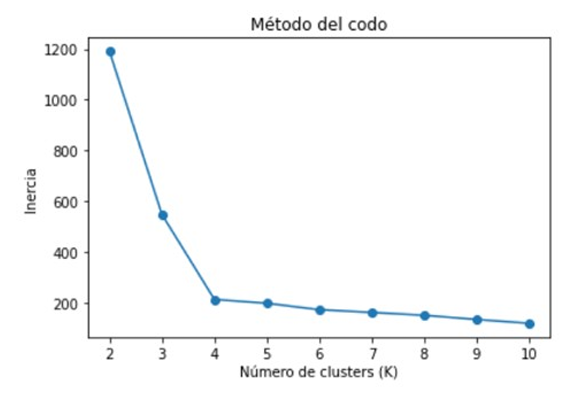
\includegraphics[width=0.85\linewidth]{imagenes/metodo-codo.png}
    \label{fig:metodo-codo}
\end{figure}

Sin embargo, este método puede ser muy subjetivo.

\subsubsection{El coeficiente de la silueta}
\begin{definition}
    El coeficiente de la silueta nos muestra un resumen de la variación dentro de un grupo y la variación entre grupos. Para cada observación, se calcula la distancia al centroide del grupo al que pertenece y lo denominamos $a$. Además, calculamos la distancia al segundo mejor centroide del grupo más cercano que no es el suyo y lo denominamos $b$. Aplicamos la siguiente fórmula:

    \begin{equation*}
        s=\dfrac{b-a}{\max(a,b)}
    \end{equation*}
\end{definition}


En un escenario ideal, la distancia $a$ es muy pequeña en comparación con la distancia $b$ por lo que el valor de $s$ es cercano a $1$; si la distancia $a$ y $b$ son similares, entonces $s$ tiende a $0$. Si la agrupación es mala, $a\ge b$ y $s$ es negativo o cercano a $-1$.

Utilizando el coeficiente de la silueta, se utiliza el método de la silueta para hallar el valor óptimo de $k$:

\begin{enumerate}
    \item Se calcula la puntuación de la silueta para cada punto del conjunto de datos.

    \item Se promedian los puntos para cada grupo.

    \item Se trazan las puntuaciones promedios para diferentes valores de $k$.

    \item El valor óptimo para $k$ es aquel en el que la puntuación de la silueta es el promedio más alto.
\end{enumerate}

\begin{figure}[ht]
    \centering
    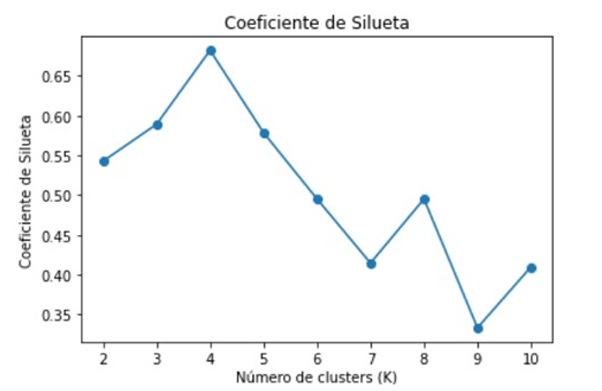
\includegraphics[width=0.85\linewidth]{imagenes/coeficiente-silueta.png}
    \label{fig:coeficiente-silueta}
\end{figure}

\subsubsection{Estadística de la brecha}

Para evaluar la calidad de los clústeres generados por K-Means, utilizamos la media de la estadística de la brecha. Esta métrica compara la inercia intra-clúster de un conjunto de datos con la que se esperaría encontrar en un conjunto de datos aleatorios sin estructura de clustering, con la inercia de los clústeres generados con los datos originales

\begin{enumerate}
    \item  \textbf{Dispersión intra-clúster con datos originales}: primero se calcula la inercia intra-clúster de los datos originales utilizando el algoritmo K-Means para diferentes valores de k. Este valor mide cuán compactos y cohesivos son los clústeres formados por el algoritmo para cada valor de k.

    \item \textbf{Dispersión intra-clúster con datos aleatorios}: se generan varios conjuntos de datos de referencia aleatorios (también conocidos como conjuntos de datos nulos)  manteniendo la estructura de los datos originales, pero mezclando aleatoriamente  las etiquetas de los puntos. Para cada conjunto de datos de referencia se calcula la  inercia intra-clúster utilizando K-Means.

    \item  \textbf{Cálculo de la brecha}: la brecha se calcula como la diferencia entre la inercia intra-clúster esperada en los datos aleatorios y la inercia intra-clúster observada en los datos originales. Se promedia esta diferencia sobre todos los conjuntos de datos de  referencia.

    \item \textbf{Selección del número óptimo de clústeres}: el número óptimo de clústeres se  elige el valor de K que maximiza la brecha. En otras palabras, se busca el punto donde la dispersión intra-clúster observada en los datos reales es menor que la dispersión de los datos aleatorios.
\end{enumerate}


\begin{figure}[ht]
    \centering
    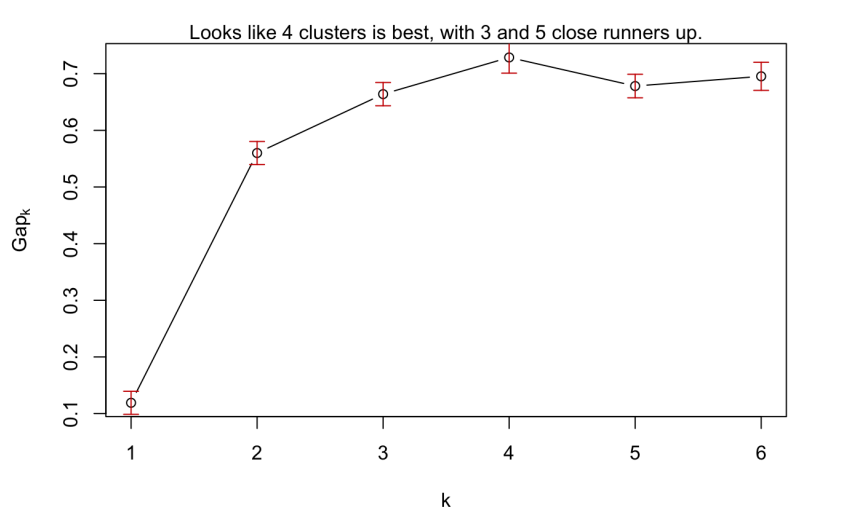
\includegraphics[width=0.85\linewidth]{imagenes/estadística-brecha.png}
    \label{fig:estadistica-brecha}
\end{figure}

\section{Ventajas y desventajas de K-Means}

\begin{table}[ht]
  \centering
  \begin{tabular}{|c|c|}
    \hline
    Ventajas de K-Means & Desventajas de K-Means \\ \hline
    Popular &  Definir el número óptimo de clústeres.\\ \hline
    Sencillo de aplicar & Sensible a \textit{outliers} \\ \hline
    Eficiencia computacional &  \\ \hline
    Puede manejar datos de alta dimensionalidad &  \\ \hline
    Escalable &  \\ \hline
    Flexible &  \\ \hline
    Fácil interpretabilidad &  \\ \hline
  \end{tabular}
  \label{tab:ventajas_desventajas-K-Means}
\end{table}

\chapter{Diferentes implementaciones de k-Means}

\section{Lloyd's K-Means}
El \textbf{algoritmo de Lloyd} es el comúnmente conocido como algoritmo \textbf{K-Means} que particiona un conjunto de datos en $K$ clústeres. Los pasos del algoritmo son los siguientes:

\begin{enumerate}
    \item Inicializa los centroides.
    \item En cada iteración:
    \begin{itemize}
        \item Asigna un punto al clúster más cercano.
        \item Calcula nuevos centroides.
        \item Verifica si los centroides han cambiado significativamente (convergencia).
    \end{itemize}

    \item Finaliza cuando los centroides ya no cambian significativamente o se alcanza el número máximo de iteraciones.

    
\end{enumerate}



\section{MacQueen's K-Means}
El problema de Lloyd's es que cuando actualiza las asignaciones de puntos de datos a clústeres, no actualiza los centroides. No tiene en cuenta que con cada actualización, el centroide cambia de posición y puede suponer que un punto esté erróneamente asignado a un centroide porque no fue actualizado.

MacQueen intenta solventar este problema actualizando los centroides con cada nueva asignación lo que también supone más tiempo de cálculo. El proceso es similar al de Lloyd's, solo que se vuelven a calcular los centroides asignados:

\begin{enumerate}
    \item Inicialización de los centroides: se comienza seleccionando aleatoriamente $K$ puntos como centroides iniciales.

    \item Asignación de puntos a centroides de manera secuencial: se calcula la distancia (euclidiana) entre cada punto del dataset y cada uno de los centroides. Se asigna el punto al centroide más cercano.

    \item Se recalculan los centroides de los clústeres después de cada asignación.

    \item Repetición: los pasos de asignación de centroides y de actualización de de estos se repiten iterativamente hasta que se converja o se alcance un número máximo de iteraciones.

    \item Convergencia.
\end{enumerate}

Diferencias entre Lloyd's y MacQueen's:

\begin{itemize}
    \item Lloyd's actualiza los centroides en pasos discretos, recalculándolos después de asignar todos los puntos de datos. Esto es más eficiente ya que se las actualizaciones se generan en un solo instante, pero requiere más iteraciones para converger debido a los cambios de centroides en cada iteración.

    \item MacQueen's actualiza los centroides de manera continua, cada vez que se asigna un punto de datos, lo que garantiza la correcta asignación del punto a un grupo de datos. Es menos eficiente que Lloyd's si estamos frente a un gran conjunto de datos, pero mejor si el flujo de datos es continuo. Converge más rápido, ya que el número de iteraciones se ajustan continuamente a los centroides.
\end{itemize}



\section{Hartigan-Wong K-Means}
Los algoritmos anteriores escogen los centroides iniciales de manera no eficiente y puede que no converja a causa de una mala inicialización.

El algoritmo de Hartigan-Wong asigna los puntos de datos a los centroides de forma aleatoria. Luego, se calcula cada centroide como la media de los puntos asignados. Así, no asocio un punto al centroide más cercano, sino al que mejor inercia da.


\begin{enumerate}
    \item Inicialización de centroides: seleccionar aleatoriamente K puntos como centroides iniciales.

    \item Al azar se asignan los puntos a un centroide.

    \item Se calcula el centroide como la media de los puntos asignados.

    \item Se repite hasta la convergencia o hasta el número máximo de iteraciones.
\end{enumerate}

\subsubsection{Diferencias entre Hartigan-Wong y Lloyd's K-Means}

\begin{itemize}
    \item En términos computacionales, Lloyd's es más simple y menos complejo que Hartigan-Wong.

    \item Hartigan-Wong requiere menos iteraciones para converger, ya que optimiza de manera continua las ubicaciones de los puntos (las actualizaciones de centroides son más frecuentes y locales al considerar la reubicación de puntos entre grupos durante las iteraciones).
\end{itemize}



\section{Elkan's K-Means}
El algoritmo de Elkan se diseñó para acelerar la convergencia de K-Means y reducir el número de cálculos de distancia necesarios. Sus principios son los siguientes:

\begin{itemize}
    \item Reducción de cálculos de distancia: Elkan utiliza los límites superiores e interiores. Elkan se basa en que si sabemos que un punto está cerca de un centroide particular, podemos evitar calcular la distancia de ese punto a otros centroides lejanos.

    \item Desigualdad triangular: evitamos calcular distancias innecesarias. La desigualdad triangular establece que, para cualquier triángulo, la suma de las longitudes de dos de sus lados será mayor o igual que la longitud del tercer lado.

    \item Actualización eficiente: cada vez que los centroides se actualizan, los límites superiores e inferiores también lo hacen, minimizando cálculos futuros.
\end{itemize}

\begin{enumerate}
    \item Inicializar los centroides de los k clústeres.

    \item Mantener un límite superior e inferior de las distancias de cada punto a los centroides. Así evitamos cálculos de distancias innecesarios.

    \item Usamos estos límites para determinar el clúster más cercano a cada punto de datos sin calcular todas las distancias.

    \item Asignar cada punto al clúster más cercano.

    \item Actualizar los centroides: calcular nuevos centroides basado en las asignaciones actuales de los puntos a los grupos.

    \item Actualización de límites: actualizar los límites superiores e inferiores tras mover los centroides.

    \item Iteración: repetir los pasos 2 a 5 hasta que se alcance la convergencia o se alcance un número máximo de iteraciones.


\end{enumerate}

\begin{itemize}
    \item Ventajas: reduce el número de cálculos de distancia.
    \item Ventajas: escalabilidad en grandes conjuntos de datos debido a la optimización de cálculos de distancia.

    \item Limitaciones: complejo de implementar.
    \item Limitaciones: sensible a la inicialización de los centroides.
\end{itemize}


\section{Soft K-Means / Fuzzy K-Means}
Uno de los grandes problemas de K-Means es su sensibilidad a la hora de inicializar los centroides. Esto se puede solventar inicializando K-Means varias veces y utilizar el valor que mejor separe a los grupos. \textbf{Soft K-Means} (o \textbf{Fuzzy K-Means}) permite que los datos pertenezcan parcialmente a múltiples grupos, en lugar de asignar cada punto estrictamente a un único grupo.

Pasos del algoritmo Soft K-Means:

\begin{enumerate}
    \item Inicialización: selección de $k$ centroides iniciales. Para cada punto $p$, se aplica una función de membresía $u$ entre 0 y 1 que indica que tan alejado/cerca está el punto $p$ del centroide del grupo. La suma de los valores de $u$ para cada punto $p$ debe ser $1$ ya que es la suma de probabilidades.

    \item Actualización de los centroides: Calculamos los centroides $C_1$ y $C_2$ en función de los valores de pertenencia. El valor centroide $C_j$ se actualiza de la siguiente manera:
    \begin{equation*}
        C_j= \dfrac{\sum_{i=1}^nu_{ij}^m.p_{i}}{\sum_{i=1}^nu_{ij}^m}
    \end{equation*}
    donde $u_{ij}$ es el valor de pertenencia elevado a la potencia $m$.

    \item Actualización de los valores de pertenencia:
    \begin{equation*}
        u_{ij}=\dfrac{1}{\sum_{k=1}^K\left(\dfrac{d(p_i,C_j)}{d\left(p_i,C_j\right)}\right)^{\dfrac{2}{m-1}}}
    \end{equation*}
    
    \item Repetir los pasos 2 y 3 hasta alcanzar la convergencia.
    
\end{enumerate}

\subsection{Otros}
\subsubsection{K-Prototype}
El objetivo de K-Prototype es poder trabajar tanto con datos numéricos como categóricos. La métrica de distancia que utiliza es mixta: euclidiana para datos numéricos y la coincidencia de categorías para categóricos. 

\section{Problema tipo de examen}

\begin{figure}[ht]
    \centering
    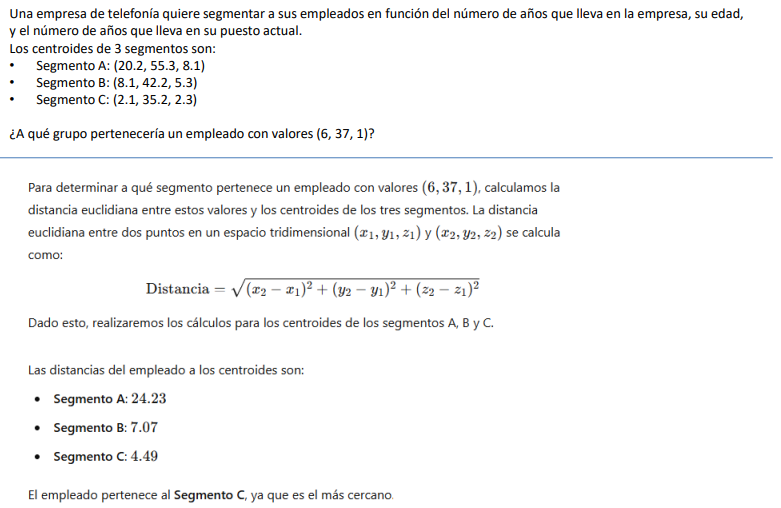
\includegraphics[width=0.95\linewidth]{imagenes/examen-clustering1.png}
    \label{fig:examen-clustering1}
\end{figure}


\begin{figure}[ht]
    \centering
    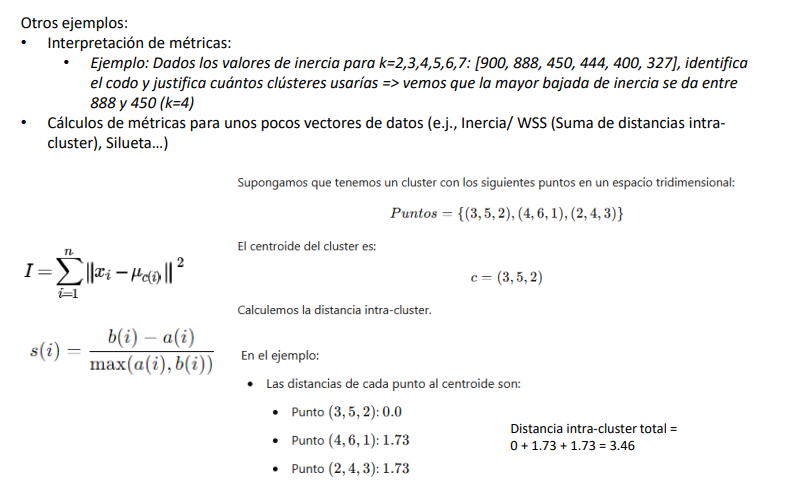
\includegraphics[width=0.95\linewidth]{imagenes/examen-clustering2.png}
    \label{fig:examen-clustering2}
\end{figure}
\chapter{Agrupamiento jerárquico}


El clustering jerárquico es un algoritmo de aprendizaje no supervisado, agrupa los  datos en jerarquía y de allí su nombre. La jerarquía se representa a través de un dendrograma o árbol que muestra las relaciones de inclusión de los diferentes
grupos. Dentro del clustering jerárquico tenemos dos grandes enfoques:

\begin{itemize}
    \item \textit{Clustering} jerárquico aglomerativo o \textit{bottom-up}.

    \item \textit{Clustering} jerárquico divisivo o \textit{top-down}.
\end{itemize}

\section{Clustering jerárquico aglomerativo o bottom-up}

Se denomina aglomerativo porque empieza con grupos muy pequeños hasta formar  un grupo. En este caso, cada punto del conjunto de datos comienza como un clúster individual, luego se combinan repetidamente en función de su similitud hasta que todos los puntos hagan parte de un solo clúster o se alcance un criterio de parada.

El funcionamiento es el siguiente:

\begin{enumerate}
    \item Primero, cada punto es un grupo en sí mismo.
    \item Luego se agrupan o dos puntos o dos grupos o un punto y un grupo cercano.
    \item Se repiten los dos pasos anteriores hasta que todos pertenezcan a un mismo grupo.
    
\end{enumerate}

\section{Clustering jerárquico divisivo o top-down}
Comienza con todos los datos en un solo clúster y se divide recursivamente en clústeres más pequeños.

El funcionamiento es el siguiente:

\begin{enumerate}
    \item Comienza guardando en un solo grupo todos los puntos.
    \item En la segunda iteración, divide el grupo en dos pequeños grupos, intenta dividir un grupo más grande en grupos más pequeños.
    \item En la tercera iteración, se divide aún más en grupos más pequeños.
    \item El algoritmo itera hasta que cada punto sea un clúster en sí mismo.
    
\end{enumerate}

\section{División de clústeres}
Lo más común es utilizar el método aglomerativo, ya que es más natural intentar agrupar en función de la similitud o distancia que intentar dividir pedazos más pequeños.

 Las secuencias de los puntos en un grupo se pueden registrar como un árbol y por eso le llamamos jerarquía. El dendrograma es un árbol que registra la secuencia de fusiones en el caso del agrupamiento aglomerativo o divisiones en el caso de agrupamiento divisivo. El número de grupos se puede elegir de manera visual.

 \begin{itemize}
     \item  calcular una matriz de proximidad, lo que significa partiendo de los puntos dados: 
     $P_1,P_2,P_3,\dots,P_n$. En la matriz se registran los valores de similitud entre cada par de puntos.
     \item Se genera un bucle con los siguientes pasos.
     \begin{enumerate}
         \item Fusión de los grupos más cercanos y registro del valor de la distancia entre los grupos en la matriz de proximidad.
         \item Se ignoran los valores de la diagonal.
         \item  Con las distancias de los diferentes clústeres creados se va creando el dendrograma.
     \end{enumerate}
     \item  Se analizan cada una de las divisiones que se pueden realizar en el dendrograma para elegir el número de clústeres ideal.
     
 \end{itemize}

\begin{figure}[ht]
     \centering
     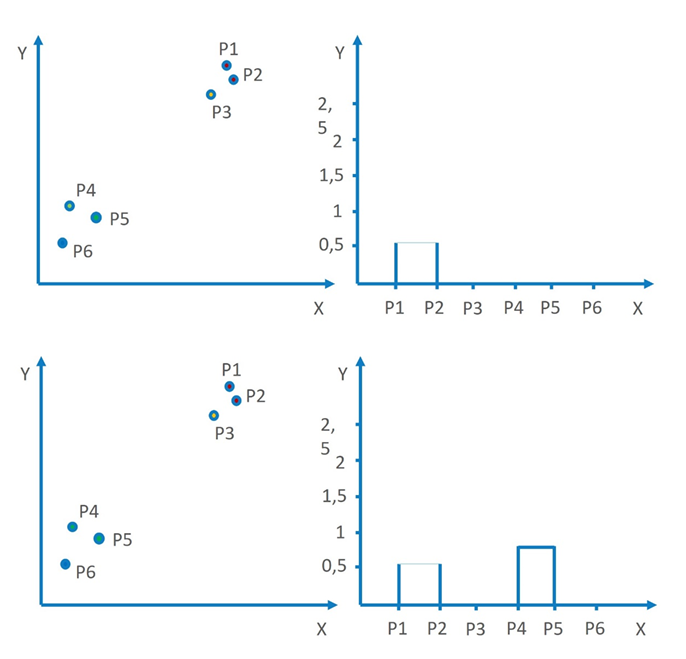
\includegraphics[width=0.5\linewidth]{imagenes/dendrograma1.png}
     \label{fig:dendrograma1}
\end{figure}

\begin{figure}[ht]
     \centering
     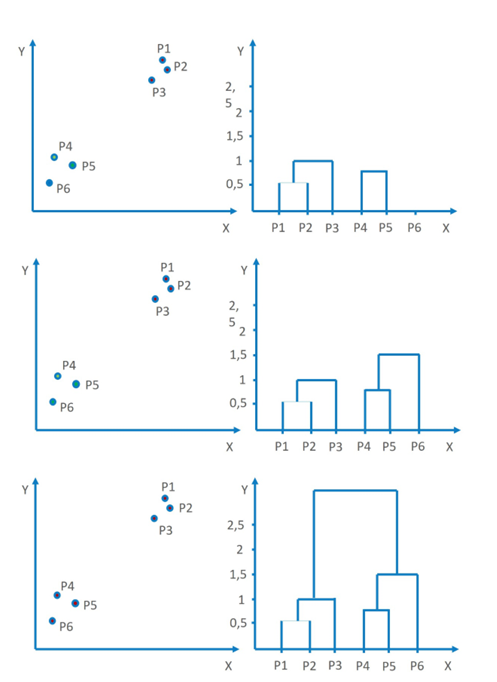
\includegraphics[width=0.5\linewidth]{imagenes/dendrograma2.png}
     \label{fig:dendrograma2}
\end{figure}

\begin{figure}[ht]
     \centering
     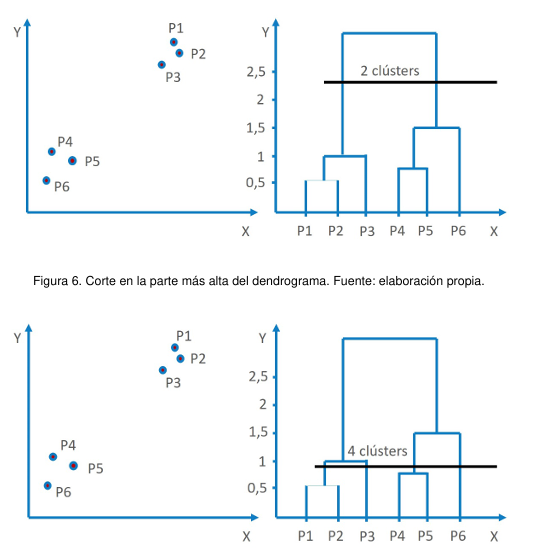
\includegraphics[width=0.5\linewidth]{imagenes/dendrograma3.png}
     \label{fig:dendrograma3}
\end{figure}

\newpage
\section{Distancias de similitud inter-clúster}
Para el ejemplo anterior, el mejor corte es el de 2 clústeres. Debido a que es la distancia más larga y garantiza la suficiente distancia inter-clúster haciendo que cada  grupo este bien diferenciado.

¿Cómo definimos la similitud inter-clúster?
\begin{itemize}
    \item Mínimo o «single linkage algorithm»: es la distancia más corta entre dos puntos que pertenezcan a los dos grupos. Este método puede manejar formas no elípticas. Su limitación es que es altamente sensible a ruido y outliers.

    \item  Máximo o «complete linkage algorithm»: calcula la distancia máxima entre cualquier par de puntos que pertenezcan a diferentes grupos. Es menos susceptible al ruido.

    \item  Media-grupal «average linkage»: calcula la distancia promedio entre todos los pares de puntos de datos que pertenecen a los diferentes grupos. Se obtiene una medida de disimilitud promedio entre grupos. Este método también es menos susceptible al ruido y a los valores atípicos.

    \item Entre-centroides: se calcula el centroide de cada grupo y se calcula la distancia entre ellos.

    \item Método Ward: es una técnica de enlace utilizada en el clustering jerárquico aglomerativo. Su objetivo principal es minimizar la varianza dentro de cada clúster. Cada punto de datos comienza como un clúster individual. En cada paso, se seleccionan los dos clústeres cuya fusión resulta en el menor incremento en la suma total de las varianzas dentro de todos los clústeres. Esta suma se calcula como la suma de las distancias cuadráticas entre cada punto y el centroide del clúster al que pertenece. El proceso de fusión se repite hasta que todos los puntos estén en un solo clúster o se cumpla un criterio de parada específico (por ejemplo, un número
 predefinido de clústeres).
\end{itemize}

\section{K-Means vs Clustering jerárquico}

\begin{figure}[ht]
    \centering
    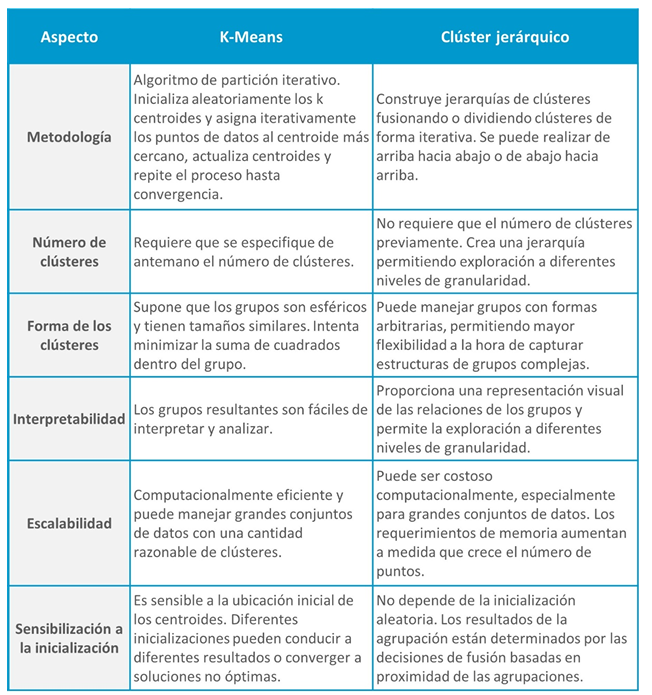
\includegraphics[width=1\linewidth]{imagenes/diferencia-kmeans-clustering-jerarquico.png}
    \label{fig:diferencia-kmeans-clustering-jerarquico}
\end{figure}

\subsection{¿Cuándo usar K-Means y cuándo agrupación jerárquica?}

\begin{itemize}
    \item K-Means funciona muy bien cuando la separación entre los grupos está bien definida. Es eficaz identificando grupos compactos o esféricos; es computacionalmente más eficiente y puede manejar gran cantidad de datos; requiere el número de clústeres previamente;  funciona muy bien con datos numéricos, gracias al manejo de distancias entre puntos; ayuda a crear prototipos y a realizar análisis exploratorio de datos; si tiene una idea de donde se pueden inicializar los clústeres, K-Means puede converger más rápido y producir resultados más precisos.

    \item El clúster jerárquico permite explorar las relaciones dentro de los datos en diferentes niveles de granularidad; es adecuado para conjuntos de datos pequeños o medianos; no requiere que el número de grupos este predeterminado; deal para datos donde existe una estructura jerárquica natural, como taxonomías biológicas, jerarquías organizacionales o relaciones genealógicas; atractivo visual informativo. 
\end{itemize}

\chapter{Clustering basado en densidades: DBSCAN}\label{TEMA5}

\section{DBSCAN}

El algoritmo \textbf{DBSCAN} (\textit{Density-Based Spatial Clustering of Applications with Noise}) es una técnica de agrupamiento no supervisada que destaca por identificar clústeres de forma arbitraria en conjuntos de datos que
 contienen ruido y distribuciones no lineales.

DBSCAN trabaja identificando regiones densas de puntos y expandiéndose a partir de estos. Además, no necesita especificar el número de clústeres iniciales. Utiliza dos parámetros principales: $\epsilon$ (épsilon), que define el radio de vecindad de un punto, y MinPts, que determina el número mínimo de puntos necesarios para formar un clúster. Un punto se considera parte de un clúster si al menos MinPts puntos caen dentro de su radio $\epsilon$.  DBSCAN tiene la capacidad de identificar puntos de datos que no pertenecen a ningún clúster.

\section{Hiperparámetros}
\begin{itemize}
    \item \textbf{Épsilon} ($\epsilon$): es la distancia máxima entre dos puntos para que se consideren vecinos el uno del otro. Es decir, si la distancia entre dos puntos es menor o igual a $\epsilon$ se consideran vecinos. Si este valor es muy pequeño, una gran parte de los datos se considerarán como valor atípico.

    \item Mínimo número de puntos: el número mínimo de puntos que debe formar un grupo denso. Como regla general, los mínimos se pueden derivar del número de dimensiones D en el conjunto de datos como mínimo número de puntos >= D+1.
\end{itemize}


En este algoritmo tenemos tres tipos de puntos de datos:

\begin{itemize}
    \item  \textbf{Punto central}: es considerado punto central si tiene más puntos MinPts dentro de los eps ($\epsilon$).

    \item  \textbf{Punto fronterizo}: un punto que tiene menos de MinPts dentro de los eps ($\epsilon$), pero que está en las proximidades de un punto central.

    \item \textbf{Ruido o valor atípico}: un punto que no es un punto central o un punto fronterizo.
\end{itemize}

\section{Pasos de DBSCAN}
\begin{enumerate}
    \item Encuentra todos los puntos vecinos dentro de eps ($\epsilon$) e identifica los puntos centrales o visitados con más vecinos teniendo en cuenta el número.
    \item  Para cada punto central, si aún no le han asignado grupo, se crea un nuevo grupo.

    \item  De manera recursiva encuentra todos los puntos conectados por densidad y asígnalos al mismo grupo que el punto central. Un punto a y b están conectados por densidad si existe un punto c que tiene un número suficiente de puntos en sus vecinos y ambos puntos a y b están dentro de la distancia $\epsilon$. Es un proceso de encadenamiento; entonces, si a es vecino de c, c es vecino de d y d es vecino de e, lo que a su vez indica que d es vecino de a, además implica que b es vecino de a.

    \item Repetir con todos los puntos restantes no visitados en el conjunto de datos. Aquellos puntos que no pertenecen a ningún grupo son considerados ruido o \textit{outliers}.
\end{enumerate}

\section{Métricas de evaluación de DBSCAN}

\subsection{Índice Rand}
 Este índice mide la similitud entre dos agrupaciones (clústeres) de un conjunto de datos: una agrupación «predicha» y una agrupación de referencia que puede ser una agrupación hecha por otro algoritmo de clustering. 

Definimos las siguientes cantidades: 

\begin{itemize}
     \item a: número de pares de puntos que están en el mismo clúster en ambos agrupamientos.
     \item b: número de pares de puntos que están en clústeres diferentes en ambos agrupamientos.

     \item c: número de pares de puntos que están en el mismo clúster en el agrupamiento real, pero en clústeres diferentes en el agrupamiento predicho.

     \item d: número de pares de puntos que están en el mismo clúster en el agrupamiento predicho, pero en clústeres diferentes en el agrupamiento real.
 \end{itemize}

 El índice Rand se calcula usando la siguiente fórmula:

\begin{equation*}
    \text{Índice Rand}=\dfrac{a+b}{a+b+c+d}
\end{equation*}

Se puede interpretar de la siguiente manera: cuanto más cerca esté de $1$ indica una coincidencia perfecta entre los dos agrupamientos; un valor cercano a $0$ indica que no hay acuerdo entre los dos agrupamientos; y, un valor de 0.5, indica que la similitud entre los agrupamientos es similar a la que se esperaría al azar.


\subsection{Coeficiente de la silueta}
La puntuación de silueta mide qué tan similar es un punto a los puntos de su propio clúster (cohesión) en comparación con los puntos del clúster más cercano (separación). Se define para cada punto y luego se puede promediar para todos los puntos en el conjunto de datos.

Para cada punto $i$: calculamos la \textbf{cohesión} $a_i$ que es la distancia promedio entre el punto $i$ y todos los demás puntos en el mismo clúster; la \textbf{separación} $b_i$ la distancia promedio entre el punto i y todos los puntos en el clúster más cercano diferente del suyo.

La puntuación de silueta para el punto $i$ se define como:
 \begin{equation*}
     s(i)=\dfrac{b_i-a_i}{\max(a_i,b_i)}
 \end{equation*}
definido entre -1 y 1.

Un valor cercano a 1 indica que el punto está bien agrupado; un valor cercano a -1 que el punto está mal agrupado; un valor de 0 indica que el punto está entre el límite de dos clústeres.


\section{Diferencias K-Means vs DBSCAN}
\begin{figure}[ht]
    \centering
    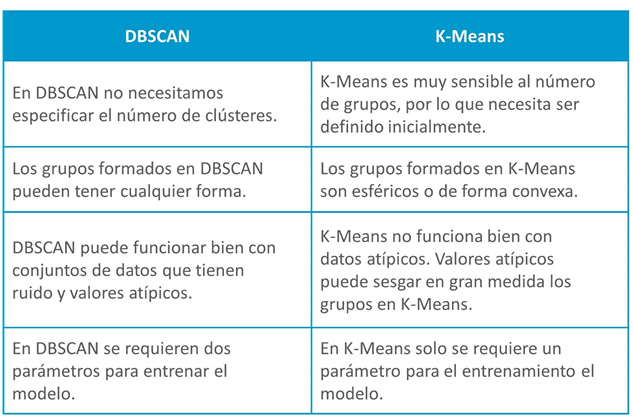
\includegraphics[width=0.85\linewidth]{imagenes/dbscan-kmeans.png}
    \label{fig:dbscan-kmeans}
\end{figure}


\section{Implementación de Python}
\subsection{KD-Tree}

Un KD-Tree (K-Dimensional Tree) es una estructura de datos en forma de árbol utilizada para organizar puntos en un espacio k-dimensional. Es particularmente útil para operaciones como la búsqueda de vecinos más cercanos y la agrupación de datos en algoritmos de aprendizaje automático y minería de datos.  Un KD-Tree es un árbol binario en el que cada nodo representa una partición de los puntos de datos en el espacio k-dimensional. Cada nodo tiene una «dimensión de corte» asociada y divide los puntos según su valor en esa dimensión

\subsection{R-Tree}
El R-Tree es una estructura de datos en forma de árbol utilizada para indexar información espacial o multidimensional. Es particularmente útil para realizar consultas espaciales eficientes, como encontrar todos los objetos dentro de una región dada. A diferencia de otros árboles, como el KD-Tree, el R-Tree está diseñado para manejar datos que no solo se representan como puntos, sino también como objetos de mayor dimensión (rectángulos, polígonos, etc.).

 
Un R-Tree está compuesto por nodos que contienen un número variable de entradas. Cada entrada en un nodo no hoja es un par formado por un identificador de nodo hijo y el MBR (Minimum Bounding Rectangle) de todos los objetos contenidos en ese nodo hijo.

\begin{itemize}
  \item Construimos un KD-Tree o un R-Tree a partir del conjunto de datos. Esto organiza los puntos de manera que las consultas espaciales sean más eficientes.
  \item Para cada punto en el conjunto de datos, en lugar de calcular la distancia a todos los otros puntos, utilizamos el árbol generado por el KD-Tree o el R-Tree para encontrar rápidamente todos los puntos dentro del radio \texttt{eps}.
  \item El KD-Tree y R-Tree permiten búsquedas eficientes en el espacio, lo que reduce el número de comparaciones y, por lo tanto, acelera el proceso de encontrar vecinos.
  \item Una vez que tenemos los vecinos, el algoritmo DBSCAN puede clasificar el punto actual como parte de un clúster, expandir el clúster o marcar el punto como ruido, según corresponda.
\end{itemize}


\begin{figure}[ht]
    \centering
    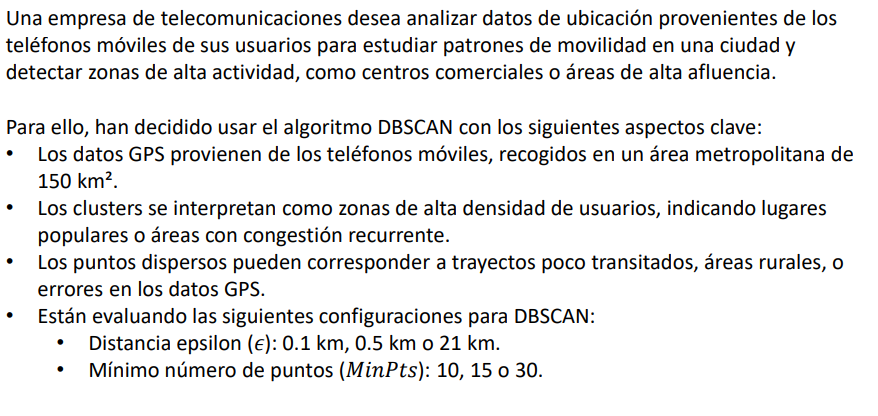
\includegraphics[width=0.85\linewidth]{imagenes/examen-dbscan1.png}
    \label{fig:examen-dbscan1}
\end{figure}


\begin{figure}[t]
    \centering
    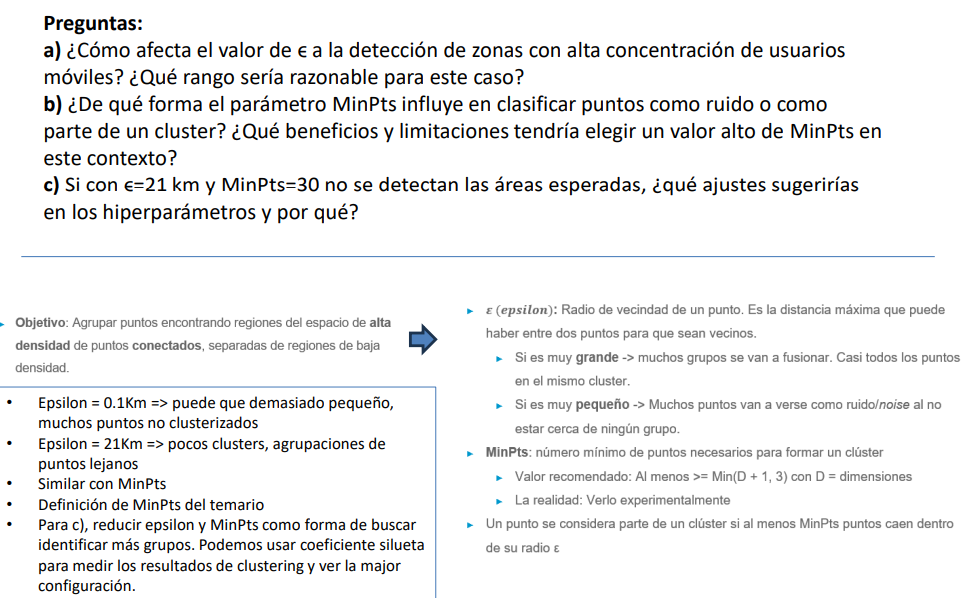
\includegraphics[width=0.85\linewidth]{imagenes/examen-dbscan2.png}
    \label{fig:examen-dbscan2}
\end{figure}
\chapter{Análisis de los Componentes Principales}

\section{¿Qué es el PCA?}
El \textbf{análisis de componentes principales} (\textit{Principal Component Analysis} - PCA) es una herramienta eficaz que ayuda a descubrir estructuras ocultas en grandes conjuntos de datos. Examina los datos complejos y multidimensionales para encontrar las perspectivas que nos den la mayor cantidad de información sobre los datos. Resalta los patrones más importantes y reduce aquellos menos importantes. El objetivo de PCA es reducir la dimensionalidad de los datos; ayuda a simplificar los datos en un conjunto más pequeño denominado «de componentes principales».


La varianza de los datos es como la diversidad de información. Una varianza alta es un indicador de que tiene una amplia gama de valores, lo que posiblemente indica una fuente rica en información. Entonces, PCA lo que hace es buscar direcciones donde esa variación sea máxima. Para elegir el primer componente principal, se intenta representar en una variable la mayor varianza posible. El segundo componente es independiente del primero; captura al igual que el primero la mayor varianza posible. Y así se crea cada uno de los componentes.

\section{Estructura matemática de PCA}
El algoritmo de PCA sigue los siguientes pasos:

\begin{enumerate}
    \item \textbf{Estandarización de datos} para garantizar que todas las características tengan la misma importancia.

    \item \textbf{Matriz de covarianza}: Es una matriz cuadrada que describe la variabilidad conjunta de dos variables. La matriz de covarianza es como una tabla que responde a la pregunta cuando una variable aumenta, ¿qué sucede con las demás? Los valores positivos indican una relación positiva (es decir, aumentan juntos), los valores negativos indican una relación negativa y cero indica que no hay relación.

    \item \textbf{Cálculo de valores y vectores propios}. Los \textbf{valores propios} (\textbf{eigenvalues}): indica cuánto estira o encoge un vector cuando se aplica una transformación lineal representada por una matriz. Los \textbf{vectores propios} (\textbf{eigenvectors}): son vectores que cuando se aplica una transformación lineal solo cambian en magnitud, no en dirección. Cada vector propio representa un componente. Lo interesante de estos vectores es que están orientados hacia donde los datos varían más.

    \item \textbf{Ordenar valores y vectores propios}. Para poder identificar los componentes principales, se deben ordenar los valores propios de forma descendente, de tal manera que mayor valor sea el primero de la lista.

    \item \textbf{Seleccionar los componentes principales}.  Se seleccionan los vectores propios con mayor valor propio. El primer componente principal corresponde al vector propio con el valor propio más grande, explicando la mayor varianza existente en el conjunto de datos. El segundo componente principal corresponde al vector propio con el segundo valor propio más grande, y así sucesivamente. El resultado es una matriz que proyecta los datos originales en un espacio de menor dimensión, reduciendo el conjunto de datos.
\end{enumerate}


\begin{figure}
    \centering
    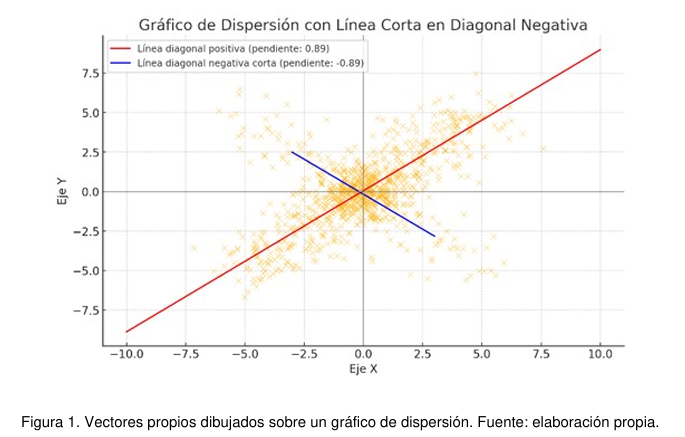
\includegraphics[width=0.5\linewidth]{imagenes/pca-grafico.png}

    \label{fig:pca-grafico}
\end{figure}


\section{Simplificación de datos}

PCA nos ofrece una solución elegante para controlar el problema de la maldición de la dimensionalidad. A medida que aumenta el número de dimensiones (características o variables) en un conjunto de datos, pueden ocurrir varios fenómenos complejos: escasez de datos, es decir, los puntos de datos tienden a estar más dispersos y para mantener la misma densidad, se necesitarían más datos; \textbf{grandes distancias entre datos} (la distancia entre puntos de datos tiende a aumentar y las diferencias entre las distancias se vuelven menos pronunciadas); la\textbf{ relevancia de las variables no es la misma}, ya que muchas puede que sean ruidosas o irrelevantes; \textbf{problemas computacionales} debido al procesamiento de datos con muchas dimensiones.


\section{Ventajas y casos de uso de PCA}
\begin{itemize}
    \item \textbf{Reducción de dimensionalidad}: al reducir el número de variables, los modelos se vuelven más simples.

    \item \textbf{Eliminación de redundancia}: ayuda a eliminar la multicolinealidad al transformar las variables originales en un nuevo conjunto de variables independientes.

    \item \textbf{Visualización en 2D y 3D}: facilita la visualización de datos complejos en dos o tres dimensiones.

    \item \textbf{Reducción de ruido}: al enfocarse en las componentes principales que captura la mayor varianza, deja de lado los componentes que representan ruido en el conjunto de datos.
\end{itemize}

Casos de uso:

\begin{itemize}
    \item \textbf{Compresión de imágenes}: al reducir la dimensionalidad de las imágenes y preservar su esencia, se pueden almacenar y transferir las imágenes.

    \item \textbf{Bioinformática}: las expresiones genéticas suelen ser conjuntos de datos de alta dimensionalidad, por lo que se puede aplicar PCA para identificar patrones y reducir el ruido. 

    \item \textbf{Reconocimiento facial}: permite la extracción de rasgos faciales esenciales para tareas de reconocimiento.

    \item \textbf{Sistemas de recomendación}: usar PCA suele obtener recomendaciones muy eficientes en datos de interacción entre un usuario y elementos en particular.
\end{itemize}

\section{Evaluación y mejora de PCA}
Existen algunos métodos para determinar el valor óptimo para el parámetro del número de componentes. Se puede realizar a través de dos visualizaciones diferentes. La primera solución es \textbf{graficar el porcentaje de varianza explicada} de los componentes individuales y el porcentaje de varianza total que capturan todos los componentes principales.

\begin{figure}[ht]
    \centering
    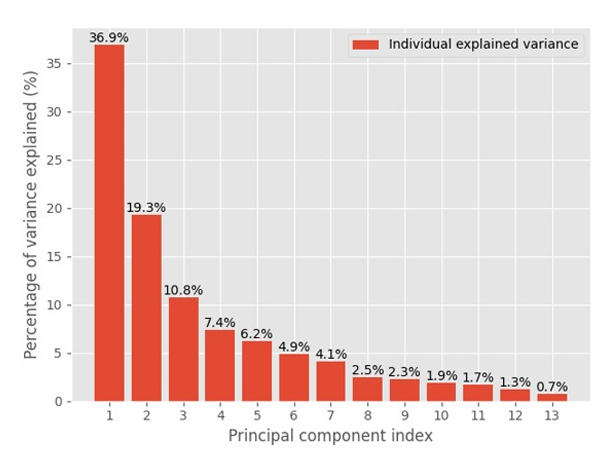
\includegraphics[width=0.75\linewidth]{imagenes/pca-grafica1.png}
    \label{fig:pca-grafica1}
\end{figure}

La segunda visualización es utilizar la técnica del codo utilizando el porcentaje de varianza explicada frente al número de componentes principales. Para poder decidir cuál es el número de componentes principales ideal.

\begin{figure}
    \centering
    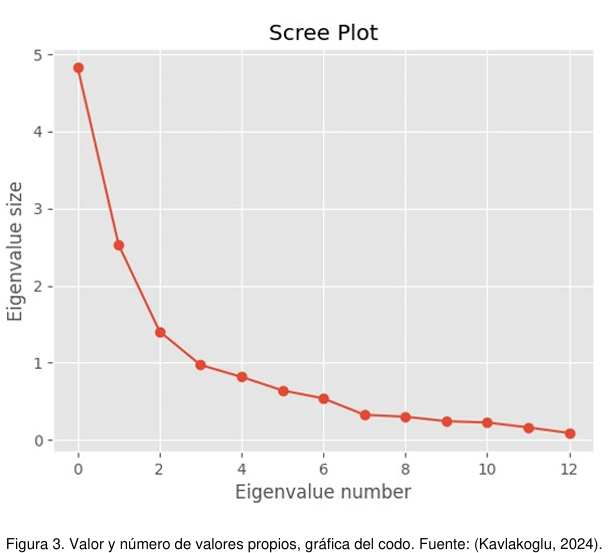
\includegraphics[width=0.75\linewidth]{imagenes/pca-grafica2.png}
    \label{fig:pca-grafica2}
\end{figure}


\chapter{Técnicas no lineales. t-SNE, MDS e ISOMAP}

\section{t-SNE (t-Distributed Stochastic Neighbor Embedding)}

\textbf{t-SNE} (\textit{t-Distributed Stochastic Neighbor Embedding}) permite transformar datos de múltiples dimensiones a representaciones bidimensionales o tridimensionales, facilitando la identificación de estructuras y relaciones intrínsecas que serían difíciles de observar en su espacio original.

La idea central de t-SNE es mapear los puntos de datos de alta dimensionalidad en un espacio de menor dimensionalidad, preservando las relaciones locales entre los puntos. Se mide la similitud entre puntos de datos en el espacio de dimensión alta y se representa dicha similitud en función de sus probabilidades. Una vez se tienen las distancias se construye una distribución de probabilidad similar en el espacio de dimensiones inferiores y se minimiza la diferencia entre las dos distribuciones utilizando la técnica del descenso del gradiente. De esta forma se captura de manera efectiva la estructura local de los datos, lo que hace particularmente útil la visualización de datos complejos y el descubrimiento de patrones.

Cuando se habla de preservar las relaciones entre los puntos, se refiere a mantener las distancias relativas y las similitudes entre puntos de datos vecinos cuando se asignan desde un espacio de alta dimensionalidad a un espacio de menor dimensión.

\subsection{Algoritmo de t-SNE}
\begin{enumerate}
    \item Selección del conjunto de datos.
    \item Preprocesamiento y normalización de los datos.

    \item Cálculo de distancias en la dimensión original: t-SNE utiliza probabilidades. Para cada punto de datos, se traza una distribución gaussiana a su alrededor con una media cero y una desviación estándar que se determina en función de la densidad de los puntos cercanos alrededor de un punto $x_1$. En un análisis de datos, se usa el eje X para representar las distancias entre cada punto del conjunto de datos y un punto de referencia específico. En el eje Y se representa la densidad de probabilidad, que indica qué tan probable es que un punto esté a cierta distancia del punto de referencia, utilizando una función de densidad para calcular una puntuación de similitud. Este proceso se repite para todos los puntos del conjunto de datos, generando una matriz de similitudes entre puntos. La distribución de probabilidades es única para cada punto, y las similitudes no son necesariamente simétricas. Un valor alto de probabilidad entre dos puntos indica que están cerca (son vecinos), y un valor bajo que están lejos.


    \item Distribución de probabilidades t-Student: para reducir la dimensionalidad, se distribuyen puntos aleatoriamente en el eje $X$. Se calcula la puntuación de similitud de cada punto con relación a los demás, obteniendo otra matriz de $n\times n$. 


    \item Con las dos matrices de $n \times m$, donde una representa las puntuaciones de similitud en la dimensión superior y la otra representa las puntuaciones de similitud en una dimensión inferior, se define una función de coste basada en la divergencia de Kullback-Leibler entre las distribuciones de alta y baja dimensión. Se alinean la matriz de dimensión inferior con la de dimensión superior, utilizando técnicas de optimización como el descenso del gradiente, para minimizar la función de coste. Esto implica ajustar la posición de los puntos de forma iterativa hasta que la matriz de similitud en la dimensión inferior se parezca lo máximo posible a la de dimensión superior. Dicho de otra forma, se itera hasta que las posiciones de los puntos en el espacio de baja dimensión converjan a una configuración que minimice la función de coste

    
    \item  Visualización y análisis: se generan visualizaciones de los datos en el espacio de baja dimensión, interpretando los resultados y analizando las agrupaciones formadas.
\end{enumerate}


\subsection{Aplicaciones de t-SNE}
\begin{itemize}
    \item Agrupación y clasificación: agrupar puntos de datos similares en dimensiones inferiores. Se suele utilizar para encontrar patrones en los datos.

    \item Detección de anomalías.

    \item Procesamiento del lenguaje natural: visualiza incrustaciones de palabras generadas a partir de un gran corpus de texto que facilita la identificación de similitudes y relaciones entre palabras.

    \item Seguridad informática: se pueden visualizar patrones de tráfico de red y detectar anomalías.

    \item Investigación del cáncer: para visualizar perfiles moleculares de muestras de tumores e identificar subtipos de cáncer.

    \item Interpretaciones geológicas: visualización de atributos sísmicos e identificación de anomalías geológicas.

    \item Procesamiento de señales biomédicas: para visualizar electroencefalogramas y detectar patrones de actividad cerebral.
\end{itemize}

\subsection{Ventajas y desventajas}
\begin{itemize}
    \item Ventajas: Si se aplica correctamente, puede ofrecer visualizaciones muy intuitivas preservando la estructura local de los datos en las dimensiones inferiores.

    \item Desventajas:  Es costoso computacionalmente. No es muy bueno preservando la estructura global. Sensible a hiperparámetros. Puede quedarse atascado en los mínimos locales. La interpretación puede ser un desafío.
\end{itemize}

\section{t-SNE vs PCA}

Ambas son técnicas de reducción de la dimensionalidad. PCA funciona mejor con datos lineales; busca identificar los componentes principales subyacentes en los datos proyectándolos en dimensiones inferiores, minimizando la variación y preservando grandes distancias por pares. t-SNE se preocupa por preservar pequeñas distancias por pares, mientras que PCA se enfoca en mantener grandes distancias por pares para maximizar la varianza.

\section{Multi-Dimensional Scaling (MDS)}
El \textbf{escalado multidimensional (MDS)} es una herramienta estadística que ayuda a descubrir conexiones entre puntos en un espacio de dimensiones más bajo que las dimensiones originales. Utiliza técnicas de análisis de datos de similitud o disimilitud canónica.

El objetivo principal es mantener las proximidades originales entre conjuntos de datos; los datos más similares se ubican muy cerca unos de otros, mientras que los datos más separados se colocan separados en el espacio de dimensión menor.

Existen tres tipos de escala multidimensional: 
\begin{itemize}
    \item  \textbf{Algoritmo clásico}: toma una matriz de entrada que representa diferencias entre pares de elementos y produce una matriz de coordenadas que minimiza la dimensionalidad.

    \item Escalamiento multidimensional métrico que generaliza el procedimiento de optimización a varias funciones de pérdida y matrices de entrada con distancias y pesos desconocidos. Minimiza una función de coste llamada «stress».

    \item  Escalado multidimensional no métrico: encuentra la relación monótona no paramétrica entre las diferencias y distancias euclidianas entre elementos, junto con la ubicación de cada elemento en el espacio de baja dimensionalidad. Se define una función de «stress» a optimizar y se considera que es monótonamente creciente.
\end{itemize}


\section{Isometric mappping (Isomap)}

Mapeo isométrico o Isomap combina varios algoritmos que le permiten utilizar una forma no lineal para reducir las dimensiones preservando las estructuras locales. 

\subsection{Algoritmo de Isomap)}

\begin{enumerate}
    \item Se utiliza KNN para encontrar los $K$ vecinos más cercanos de cada punto del conjunto de datos.
    \item Se construye un grafo de vecindad conectando solo los puntos que son vecinos; los demás quedan desconectados.
    \item Se calcula la distancia geodésica entre todos los pares de puntos usando algoritmos como Floyd-Warshall o Dijkstra.
    \item Se aplica escalado multidimensional (MDS) para incrustar los puntos en un espacio de menor dimensión, preservando las distancias geodésicas.
\end{enumerate}


\section{Comparativa de todas las técnicas de reducción de dimensionalidad}

\begin{figure}[ht]
    \centering
    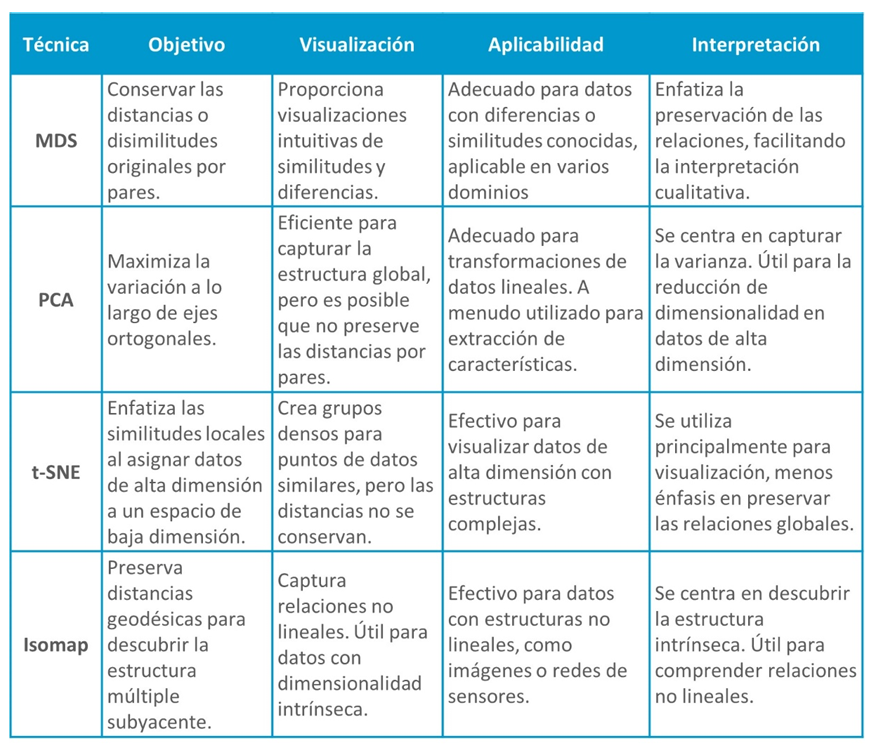
\includegraphics[width=1\linewidth]{imagenes/comparativa-reduccion-dim.png}
    \label{fig:comparativa-reduccion-dim}
\end{figure}
\chapter{Detección de anomalías}

\section{¿Qué es la detección de anomalías?}
 La detección de anomalías combina las técnicas de aprendizaje supervisado para generar un modelo de valores normales y, posteriormente, se utiliza este modelo con nuevos registros para detectar valores anómalos o inusuales.
 
 
Una anomalía es una observación que se desvía del comportamiento o patrón esperado de un conjunto de datos determinado. Estas técnicas también se conocen en la literatura con el nombre de detección de \textit{outliers}. En esencia, un \textit{outlier} es un valor poco habitual y, por tanto, puede ser considerado una anomalía.

\subsection{Técnicas para detectar anomalías}
\begin{itemize}
    \item \textbf{Detección de anomalías con algoritmos supervisados}: se utilizan datos etiquetados para entrenar un modelo que incluye instancias normales y anómalas.

    \item \textbf{Detección de anomalías con algoritmos no supervisados}: el modelo aprende a identificar anomalías sin conocimiento previo de lo que constituye un comportamiento normal.

    \item \textbf{Detección de anomalías con algoritmos semisupervisados}: el modelo aprende a identificar anomalías en los datos sin etiquetar en función de lo que aprende de los datos etiquetados.

    \item Detección estadística de anomalías: utilizando técnicas estadísticas para detectar anomalías basadas en la distribución de los datos.
\end{itemize}

\subsection{Tipos de outliers}

\begin{itemize}
    \item Valor atípico global: hay una desviación significativa del resto de datos.

    \item  Valor atípico contextual: el objeto se desvía significativamente según un contexto seleccionado. 

    \item Valor atípico colectivo: cuando un subconjunto de datos en un conjunto se desvía del conjunto completo, incluso si los objetos de datos individuales pueden no ser valores atípicos.
\end{itemize}

\subsection{Ventajas y desventajas}
\begin{itemize}
    \item Ventajas: detección temprana de anomalías; precisión mejorada; seguridad y eficiencia mejoradas.

    \item Desventajas: detectar datos normales como valores atípicos (falsos positivos); preprocesamiento de datos necesario; la selección del modelo es crítico; los datos han de estar equilibrados.
\end{itemize}


\section{Métodos estadísticos para la detección de anomalías}

Los métodos estadísticos univariables se centran en el análisis de una sola variable a la vez. Estos métodos incluyen técnicas como el cálculo de la media y la desviación estándar para identificar valores que se desvían significativamente del comportamiento esperado, el uso del Z-Score para estandarizar las puntuaciones y detectar outliers, así como la aplicación de la media móvil para observar tendencias y detectar irregularidades a lo largo del tiempo.

En el ámbito de la estadística, las pruebas son fundamentales para la toma de decisiones y la prueba de hipótesis. Se utilizan pruebas paramétricas y no paramétricas para discernir patrones y relaciones importantes en los datos.

\subsection{Pruebas no paramétricas}

Las pruebas no paramétricas son útiles para detectar anomalías especialmente cuando no se pueden hacer suposiciones sobre la distribución de los datos. 

\subsubsection{Método del percentil}

El método del percentil define un umbral con base en el rango percentil de los puntos de datos. Identificar anomalías como valores que están por debajo o por encima de un percentil específico es útil cuando se trata de distribuciones asimétricas no gaussianas.

\subsubsection{Método de la media móvil}
Este método calcula la media móvil de los puntos de datos y compara cada dato con la media. Las anomalías suelen estar desviados significativamente del promedio móvil.


Existen otras pruebas no paramétricas comunes para la detección de anomalías: test de Grubbs (test de Grubbs para un outlier), test de Tukey (prueba de rango intercuartílico), test de Wilcoxon (test de Wilcoxon para muestras apareadas), test de Kruskal-Wallis y test de Mann-Whitney U. 

\subsection{Pruebas paramétricas}

Estas técnicas se basan en parámetros estadísticos como la media y la desviación estándar para identificar puntos de datos que se desvían significativamente de la norma.

Cada prueba actúa sobre un escenario diferente, por ejemplo, Z-Score y T-Score se utilizan para comparar las medias de uno o dos grupos; ANOVA se utiliza para comparar las medias de tres o más grupos.

\subsection{Z-Score}
El Z-Score es una técnica estadística que nos permite detectar anomalías. Si el valor de Z para un punto de datos supera el umbral establecido por el usuario de $x$ desviaciones estándar que se alejan de la media, se considera anomalía.

\subsection{T-Score}
La prueba de T-Score es similar al Z-Score, pero se utiliza cundo el tamaño de la muestra es pequeño y la desviación estándar es desconocido.


\section{Algoritmos basados en distancia}

La idea principal de los algoritmos basados en distancia es que los puntos de datos que están lejos de otros puntos se consideran anomalías. Se basan en los siguientes principios:

\begin{itemize}
    \item  Distancia euclidiana.
    \item Distancia al vecino más cercano: los puntos de datos que tienen una distancia mayor que un umbral a su vecino más cercano se consideran anomalías.

    \item Distancia media a k-vecinos más cercanos: similar a la anterior, pero usa la media de la distancia de los k-vecinos más cercanos.
\end{itemize}

\subsection{Métodos comunes basados en distancia}
\subsubsection{K-Nearest Neighbors (k-NN)}
Detecta anomalías basándose en la distancia a los k vecinos más cercanos.
Funcionamiento: calcula la distancia de cada punto a sus k vecinos más cercanos. Se define un umbral de distancia. Los puntos cuya distancia a sus k vecinos más cercanos excede el umbral se consideran anomalías

\subsubsection{Distance-Based Outlier Detection (DBOD)}
Detecta anomalías considerando la distancia a un conjunto de vecinos.

Funcionamiento: para cada punto, encuentra sus k vecinos más cercanos. Se calcula la distancia al vecino más cercano y a otros vecinos. Los puntos con las mayores distancias son considerados anomalías.

\subsubsection{Distancia de Mahalanobis}

Utiliza la distancia de Mahalanobis para detectar anomalías en datos multivariados considerando la correlación entre variables.

Funcionamiento: aplica un algoritmo de clustering para agrupar los datos. Calcula la distancia de cada punto al centroide de su clúster. Los puntos con grandes distancias a sus centroides son considerados anomalías.


\section{Algoritmos basados en densidad}
Los algoritmos basados en densidad identifican anomalías detectando puntos en el espacio de datos que están en regiones de baja densidad. Los puntos de datos que no tienen suficientes vecinos cercanos o están significativamente alejados de otros puntos se consideran anomalías.

Tienen en cuenta que la densidad local de un punto se calcula considerando su proximidad a otros puntos. Los puntos en áreas de baja densidad se consideran anomalías

 Los algoritmos más comunes son: Local Outlier Factor (LOF), Density-Based Spatial Clustering of Applications with Noise (DBSCAN) (ver \hyperref[TEMA5]{TEMA 5. DBSCAN}) y One-Class SVM con Kernel Gaussiano (RBF).

\subsection{Local Outlier Factor (LOF)}
El LOF mide la densidad local de un punto en comparación con la densidad de sus vecinos más cercanos. Detecta anomalías en datos de alta dimensión y en clústeres de diferentes densidades.

Funcionamiento:  

\begin{itemize}
    \item  Distancia k-vecino más cercano: para cada punto, se calcula la distancia al k-ésimo vecino más cercano.
    \item Densidad local: se calcula la densidad local de un punto como la inversa de la distancia promedio a sus k-vecinos más cercanos.
 
    \item Factor de outlier local (LOF): compara la densidad local del punto con la densidad local de sus vecinos. Un LOF significativamente mayor que 1 indica una anomalía.
\end{itemize}

\section{Isolation Forest}

Isolation Forest es un método basado en árboles de decisión, similar al Random Forest. La idea principal del Isolation Forest se basa en que las anomalías son datos «poco frecuentes» y «diferentes» que se aíslan fácilmente. Es decir, se necesitan pocas particiones para aislar una anomalía.

Funcionamiento:

\begin{itemize}
    \item Se generan múltiples árboles de aislamiento de forma aleatoria.
    \item En cada nodo del árbol se selecciona aleatoriamente una característica (dimensión) y un valor de corte para dividir el espacio.
    \item Este proceso se repite recursivamente hasta que cada punto quede aislado o se alcance una profundidad máxima.
    \item Las observaciones que requieren menos divisiones (profundidad baja) para quedar aisladas se consideran más anómalas.
    \item La puntuación de anomalía de una instancia se calcula como la \textbf{profundidad media} a la que es aislada en todos los árboles. Cuanto menor sea esta media, mayor es la probabilidad de que se trate de una anomalía.
\end{itemize}

El algoritmo es eficiente para conjuntos de datos grandes y de alta dimensión, ya que no requiere suposiciones estadísticas sobre la distribución de los datos.



\chapter{Introducción al aprendizaje por refuerzo}

\section{Aprendizaje por refuerzo y agentes}
El \textbf{aprendizaje por refuerzo} (\textit{reinforcement learning}, RL) es una rama del aprendizaje automático que se centra en cómo los agentes deben tomar decisiones para maximizar alguna noción de recompensa acumulada a lo largo del tiempo. A diferencia de otros enfoques de aprendizaje, el RL permite a los agentes aprender a través de la interacción directa con su entorno, ajustando sus estrategias en función de las consecuencias de sus acciones.

Los \textbf{agentes} se definen como programas de software capaces de operar de manera autónoma, percibiendo su entorno mediante sensores y actuando sobre él mediante actuadores.

Un agente inteligente se define por las siguientes propiedades fundamentales:

\begin{itemize}
    \item \textbf{Autonomía:} opera sin intervención humana directa, controlando sus propias acciones y estado interno.
    \item \textbf{Percepción y acción:} recoge información del entorno mediante sensores y actúa sobre él mediante actuadores.
    \item \textbf{Objetivo o función de recompensa:} tiene un criterio claro de éxito que guía su comportamiento.
    \item \textbf{Adaptabilidad:} modifica su comportamiento a partir de experiencias previas o nueva información.
    \item \textbf{Persistencia:} actúa de forma continua a lo largo del tiempo.
\end{itemize}

\subsection*{Tipos de agentes inteligentes}

Existen varios tipos de agentes según su complejidad y modelo de decisión:

\begin{itemize}
    \item \textbf{Agente reactivo simple:} responde directamente a las percepciones actuales sin tener en cuenta el historial. \\
    \textit{Ejemplo:} un termostato.
    
    \item \textbf{Agente basado en modelo:} mantiene una representación interna del entorno para tomar decisiones más informadas. \\
    \textit{Ejemplo:} un robot de limpieza que recuerda obstáculos.

    \item \textbf{Agente basado en objetivos:} actúa para alcanzar objetivos específicos, no solo para reaccionar. \\
    \textit{Ejemplo:} un agente de búsqueda en un videojuego.

    \item \textbf{Agente basado en utilidad:} toma decisiones optimizando una función de utilidad que puede incorporar múltiples objetivos y prioridades. \\
    \textit{Ejemplo:} un sistema de recomendación personalizado.
\end{itemize}

\section{Procesos de decisión de Markov (MDP)}

Un MDP es un marco matemático utilizado para modelar la toma de decisiones en situaciones donde los resultados son en parte aleatorios y en parte bajo el control de un agente.

Son esenciales en el RL porque proporcionan la estructura matemática para modelar y resolver problemas en los que un agente debe aprender a tomar decisiones óptimas a través de la interacción con su entorno.

Se compone de:

\begin{itemize}
    \item \textbf{Estados (S):} representan todas las posibles situaciones en las que puede encontrarse el agente.
    
    \item \textbf{Acciones (A):} conjunto de todas las acciones posibles que el agente puede realizar en cada estado.
    
    \item \textbf{Transiciones (T):} definen la probabilidad de pasar de un estado a otro al realizar una acción específica. \\
    Formalmente, $T(s, a, s') = P(s' \mid s, a)$, donde:
    \begin{itemize}
        \item $s$ es el estado actual,
        \item $a$ es la acción tomada,
        \item $s'$ es el estado siguiente.
    \end{itemize}
    
    \item \textbf{Recompensas (R):} cuantifican la ganancia inmediata tras transitar de un estado a otro por medio de una acción. \\
    Formalmente, $R(s, a, s')$ es la recompensa recibida al pasar de $s$ a $s'$ mediante la acción $a$.
    
    \item \textbf{Política ($\pi$):} es la estrategia que sigue el agente para decidir qué acción tomar en cada estado. \\
    Puede representarse como $\pi(a \mid s)$, que indica la probabilidad de tomar la acción $a$ en el estado $s$.
\end{itemize}

\subsection*{Política óptima y política estacionaria}

\begin{itemize}
    \item \textbf{Política óptima ($\pi^*$):} es la estrategia que maximiza el rendimiento esperado a largo plazo desde cualquier estado inicial. Representa la mejor política que un agente puede seguir para obtener el mayor beneficio esperado.

    \item \textbf{Política estacionaria:} es aquella en la que la decisión del agente depende únicamente del estado actual y no del instante de tiempo. \\
    Esto implica que si el agente se encuentra varias veces en un mismo estado, ejecutará siempre la misma acción, independientemente del momento. \\
    Las políticas estacionarias simplifican el análisis y la implementación en algoritmos de aprendizaje por refuerzo.
\end{itemize}

\subsection*{Utilidad}

La utilidad es una medida del valor o satisfacción que un agente obtiene a partir de una secuencia de decisiones o resultados. Se utiliza para evaluar y comparar distintas políticas.

\begin{itemize}
    \item \textbf{Utilidad aditiva:} el valor total de una trayectoria se calcula como la suma directa de las recompensas recibidas en cada paso:
    \[
    U = \sum_{t=0}^{T} R_t
    \]

    \item \textbf{Utilidad ponderada:} cada recompensa se multiplica por un factor de ponderación $\omega_t$, permitiendo priorizar ciertas decisiones:
    \[
    U = \sum_{t=0}^{T} \omega_t \cdot R_t
    \]

    \item \textbf{Utilidad descontada:} las recompensas futuras se reducen en valor mediante un factor de descuento $\gamma \in [0,1)$. Es ampliamente utilizada en aprendizaje por refuerzo:
    \[
    U = \sum_{t=0}^{\infty} \gamma^t \cdot R_t
    \]
    Este enfoque permite equilibrar entre recompensas inmediatas y futuras.
\end{itemize}

La \textbf{utilidad total} en un proceso de decisión secuencial se define como la suma de las recompensas futuras descontadas. Este concepto es clave en el aprendizaje por refuerzo, ya que permite al agente equilibrar la \textit{explotación} de recompensas inmediatas con la \textit{exploración} de recompensas futuras.

Formalmente, si $R_t$ representa la recompensa obtenida en el instante $t$, y $\gamma \in [0,1)$ es el factor de descuento, entonces la utilidad total $U$ se expresa como:

\[
U = \sum_{t=0}^{\infty} \gamma^t \cdot R_t
\]

Este modelo de utilidad es utilizado en algoritmos fundamentales del aprendizaje por refuerzo, como el \textbf{Q-learning} y los algoritmos basados en \textbf{política de valor}.


\section{Ecuaciones de Bellman}
Las \textbf{ecuaciones de Bellman} proporcionan una formulación matemática que descompone un problema de decisión secuencial en subproblemas más simples. Son fundamentales tanto en optimización dinámica como en aprendizaje por refuerzo, especialmente en entornos modelados como procesos de decisión de Markov (MDP).

\subsubsection*{Conceptos clave}

\begin{itemize}
    \item \textbf{Estado ($s$):} representa la situación actual del agente.
    \item \textbf{Acción ($a$):} decisión que el agente puede tomar desde un estado determinado.
    \item \textbf{Recompensa ($r$):} beneficio inmediato obtenido al tomar una acción en un estado.
    \item \textbf{Política ($\pi$):} estrategia que define qué acción tomar en cada estado.
    \item \textbf{Valor ($V$):} utilidad esperada total que se puede obtener al partir de un estado $s$ y seguir una política determinada.
\end{itemize}

Las ecuaciones de Bellman permiten calcular recursivamente el valor de cada estado, considerando todas las recompensas futuras esperadas, lo que resulta clave para definir políticas óptimas.

La \textbf{ecuación de Bellman} para una política $\pi$ se expresa como:

\[
V^{\pi}(s) = \mathbb{E} \left[ r_t + \gamma V^{\pi}(s_{t+1}) \mid s_t = s, \pi \right]
\]

Donde:
\begin{itemize}
    \item $V^{\pi}(s)$ es el valor del estado $s$ siguiendo la política $\pi$.
    \item $r_t$ es la recompensa inmediata al tomar la acción $a$ en el estado $s$.
    \item $\gamma$ es el factor de descuento ($0 \leq \gamma < 1$).
    \item $s_{t+1}$ es el estado siguiente.
    \item La esperanza $\mathbb{E}$ se toma sobre todas las acciones y estados posibles, dado que se sigue la política $\pi$.
\end{itemize}

Las ecuaciones de Bellman permiten descomponer un problema de decisión secuencial en subproblemas más simples. Son fundamentales en algoritmos como \textit{value iteration}, \textit{policy iteration} y \textit{Q-learning}, ya que ayudan a encontrar la política óptima que maximiza la recompensa esperada a largo plazo.







\section{Aplicaciones}

\textbf{1. Conducción autónoma}

El aprendizaje por refuerzo profundo se aplica en:
\begin{itemize}
    \item Optimización de trayectorias y planificación del movimiento.
    \item Estacionamiento automático, cambio de carril con Q-learning y adelantamientos seguros.
    \item Ejemplo: \textit{AWS DeepRacer}, un coche autónomo que aprende a conducir mediante RL en una pista física.
\end{itemize}

\textbf{2. Automatización industrial}

\begin{itemize}
    \item Robots RL realizan tareas peligrosas para humanos.
    \item Ejemplo destacado: DeepMind optimiza el enfriamiento de centros de datos de Google, reduciendo un 40\% del consumo energético mediante decisiones basadas en RL.
\end{itemize}

\textbf{3. Comercio y finanzas}

\begin{itemize}
    \item RL decide cuándo comprar, vender o mantener activos.
    \item Mejora la coherencia frente a decisiones humanas.
    \item Ejemplo: plataforma financiera de IBM que calcula recompensas según ganancias o pérdidas.
\end{itemize}

\textbf{4. Procesamiento del lenguaje natural (PLN)}

\begin{itemize}
    \item Aplicaciones: resumen automático, respuesta a preguntas, traducción y generación de diálogos.
    \item Ejemplo: investigadores de Stanford y Microsoft Research utilizan RL profundo para generar conversaciones coherentes e informativas mediante agentes virtuales.
\end{itemize}

\textbf{5. Atención sanitaria}

\begin{itemize}
    \item Se aplican políticas óptimas de tratamiento sin modelos matemáticos previos.
    \item Usos en regímenes de tratamiento dinámico (DTR), diagnóstico automatizado y optimización de resultados a largo plazo.
    \item RL considera efectos retardados de los tratamientos.
\end{itemize}

\textbf{6. Ingeniería y producción a gran escala}

\begin{itemize}
    \item Ejemplo: plataforma \textit{Horizon} de Facebook, utilizada para:
    \begin{itemize}
        \item Personalizar sugerencias y notificaciones.
        \item Optimizar calidad de vídeo según el estado del buffer y condiciones de red.
    \end{itemize}
\end{itemize}

\textbf{7. Recomendación de noticias}

\begin{itemize}
    \item RL se adapta a cambios en preferencias del usuario.
    \item Se definen recompensas en función de clics, compartidos, actualidad, contexto, etc.
    \item Considera tanto características de las noticias como del lector y el entorno.
\end{itemize}



\begin{figure}[ht]
    \centering
    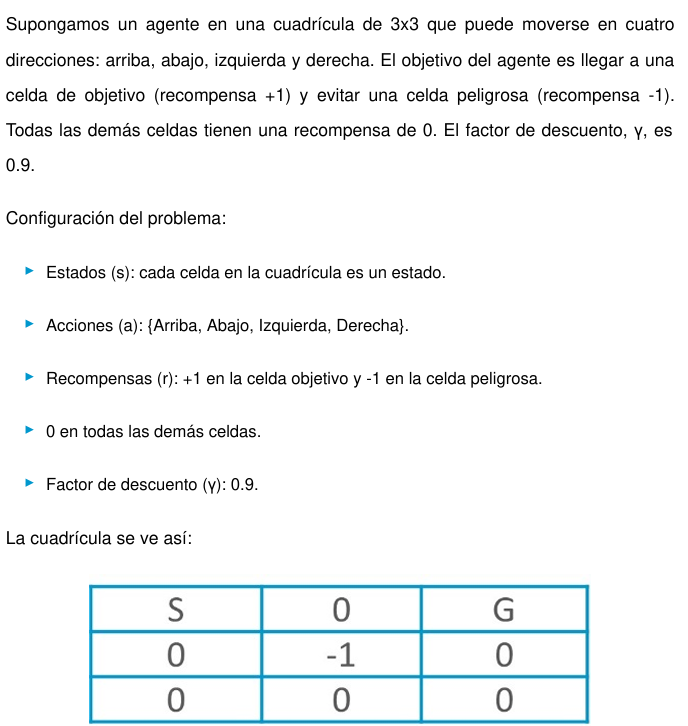
\includegraphics[width=0.55\linewidth]{imagenes/bellman1.png}

\end{figure}

\begin{figure}[ht]
    \centering
    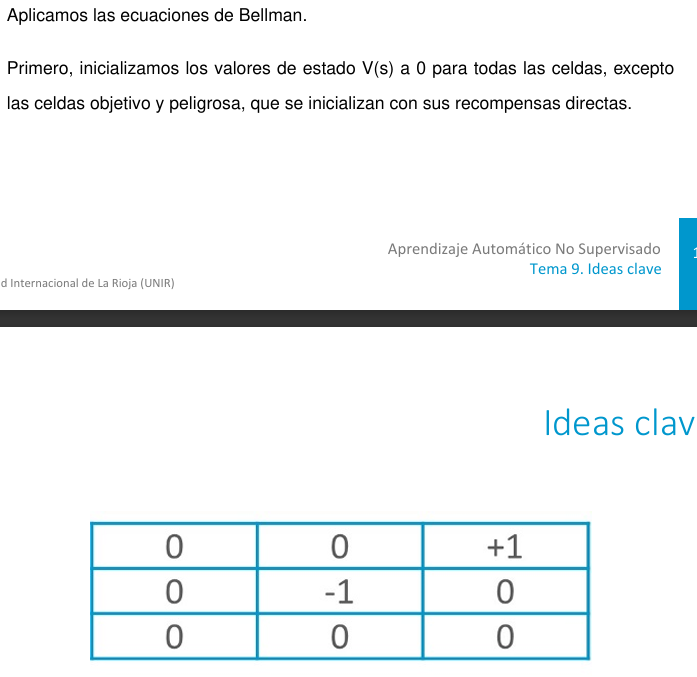
\includegraphics[width=0.55\linewidth]{imagenes/bellman2.png}

\end{figure}

\begin{figure}[ht]
    \centering
    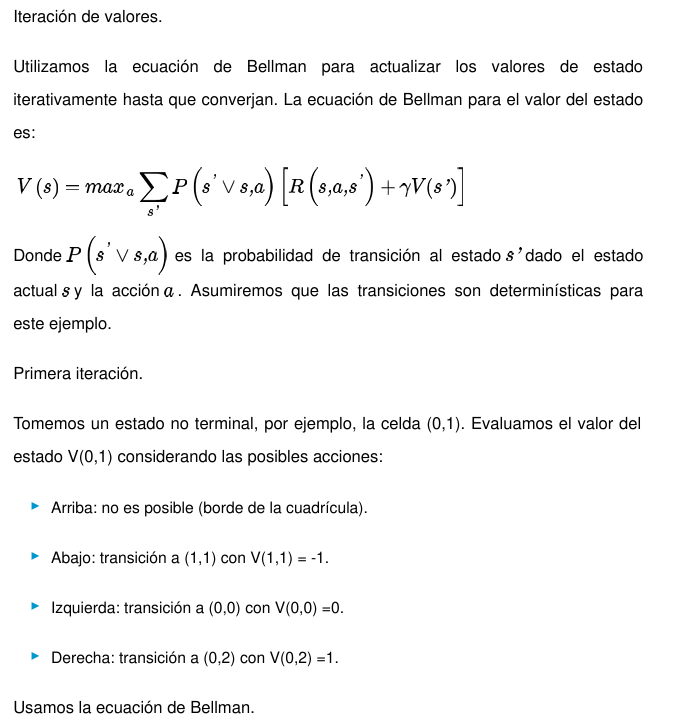
\includegraphics[width=0.55\linewidth]{imagenes/bellman3.png}

\end{figure}

\begin{figure}[ht]
    \centering
    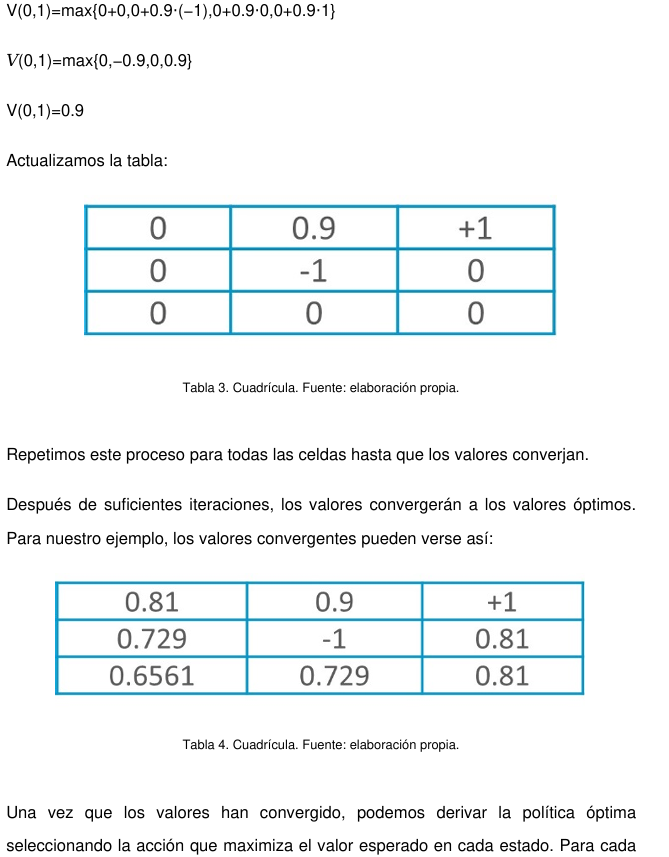
\includegraphics[width=0.55\linewidth]{imagenes/bellman4.png}

\end{figure}
\chapter{Q-Learning, DQL, Reinforce, PPO}
\section{Q-Learning}
El algoritmo de Q-learning es una técnica de aprendizaje por refuerzo que permite a un agente aprender la política óptima para tomar decisiones en un entorno determinado.

Usa TD para actualizar la función acción-valor:
\begin{itemize}
    \item Actualiza las acciones-valores en cada interacción con el entorno.
    \item No aprende una política directamente, sino que la deriva de las acciones-valores de los estados (método basado en valor).
\end{itemize}



\begin{figure}[ht]
    \centering
    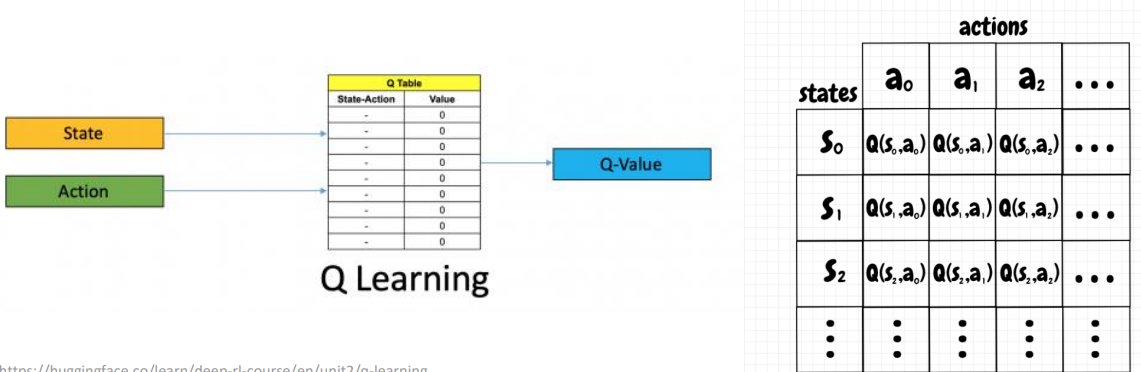
\includegraphics[width=0.75\linewidth]{imagenes/q-learning1.png}
    \label{fig:q-learning1}
\end{figure}



\begin{figure}[ht]
    \centering
    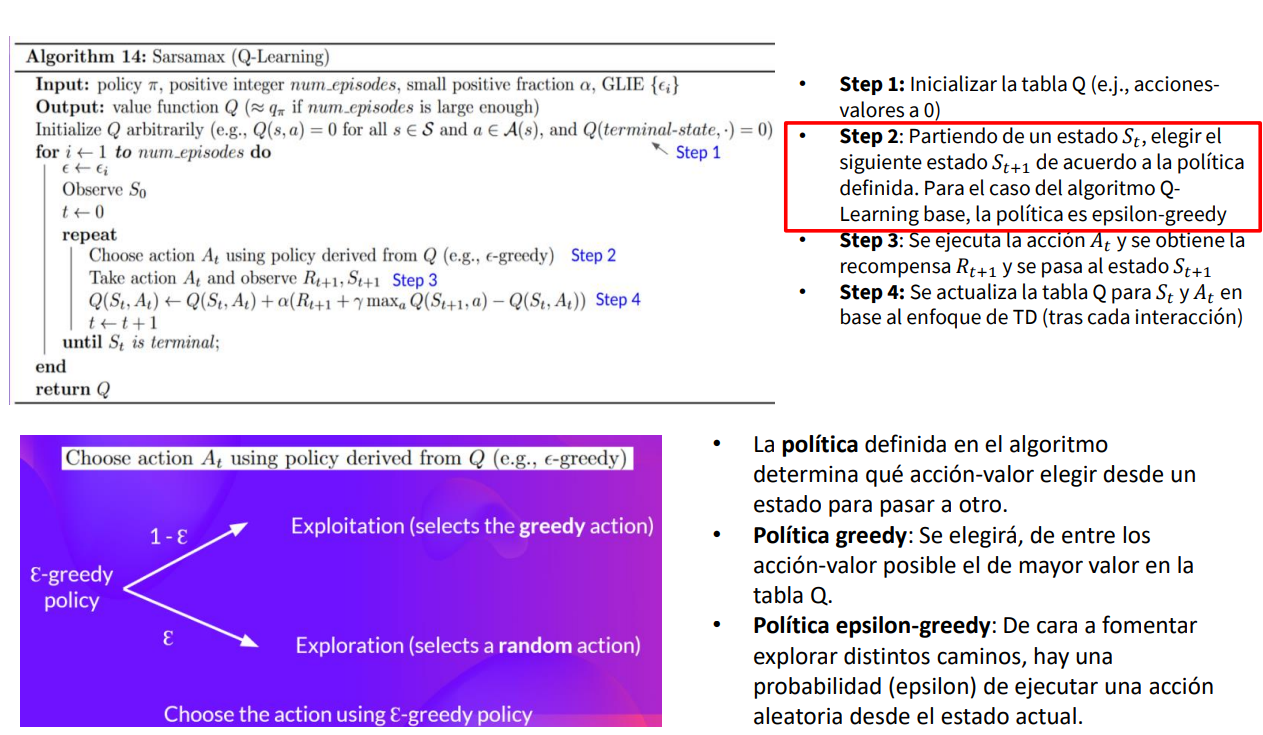
\includegraphics[width=0.75\linewidth]{imagenes/q-learning2.png}
    \label{fig:q-learning2}
\end{figure}


La fórmula de actualización se muestra en la siguiente ecuación:
\[
Q(s,a) \leftarrow Q(s,a) + \alpha \left[ r + \gamma \max_{a'} Q(s', a') - Q(s,a) \right]
\]

Donde:
\begin{itemize}
    \item $\alpha$ es la tasa de aprendizaje, que controla la actualización de los valores Q en cada paso ($0 < \alpha \leq 1$).
    \item $\gamma$ (gamma) es el factor de descuento, que determina la importancia de las futuras recompensas ($0 \leq \gamma < 1$).
    \item $R$ es la recompensa recibida después de tomar la acción $a$ en un estado $s$.
    \item $\max_{a'} Q(s', a')$ es el valor máximo de Q para el siguiente estado $s'$, considerando todas las posibles acciones $a'$.
\end{itemize}

Al ser un algoritmo de aprendizaje por refuerzo, los conceptos de estado, acción, recompensa son los mismos. Acá encontramos términos nuevos: episodio, valor óptimo de Q, estimación de Q, tabla Q y diferencias temporales.

\begin{itemize}
    \item \textbf{Episodio}: es el final de una etapa, donde los agentes no pueden emprender nuevas acciones. Se produce cuando el agente ha alcanzado el objetivo o ha fracasado.
    \item $Q(s_{t+1}, a)$: es el valor óptimo de Q esperado después de realizar la acción en un estado concreto.
    \item $Q(s_t, A_t)$: es la estimación actual de $Q(s_{t+1}, a)$.
    \item \textbf{Tabla Q}: el agente mantiene la tabla Q de conjuntos de estados-acciones.
    \item \textbf{Diferencias temporales (TD)}: se usa para estimar el valor esperado de $Q(s_{t+1}, a)$. Hace uso del estado y la acción actual y el estado y acción anterior.
\end{itemize}

\begin{center}
\begin{tikzpicture}[
  node distance=1.8cm and 3cm,
  every node/.style={draw, rounded corners, align=center, minimum width=3.5cm, minimum height=1.2cm, font=\normalsize},
  arrow/.style={-Stealth, thick}
]
\node (init) {Inicializar tabla Q};
\node (update) [right=of init] {Actualizar tabla Q};
\node (choose) [below=of init] {Escoger y ejecutar acción};
\node (reward) [right=of choose] {Medir recompensa};

\draw[arrow] (init) -- (update);
\draw[arrow] (update) -- (reward);
\draw[arrow] (reward) -- (choose);
\draw[arrow] (choose) -- (init);
\end{tikzpicture}
\end{center}


\subsection{Ejemplo}

\begin{figure}[ht]
    \centering
    \begin{minipage}{0.48\linewidth}
        \centering
        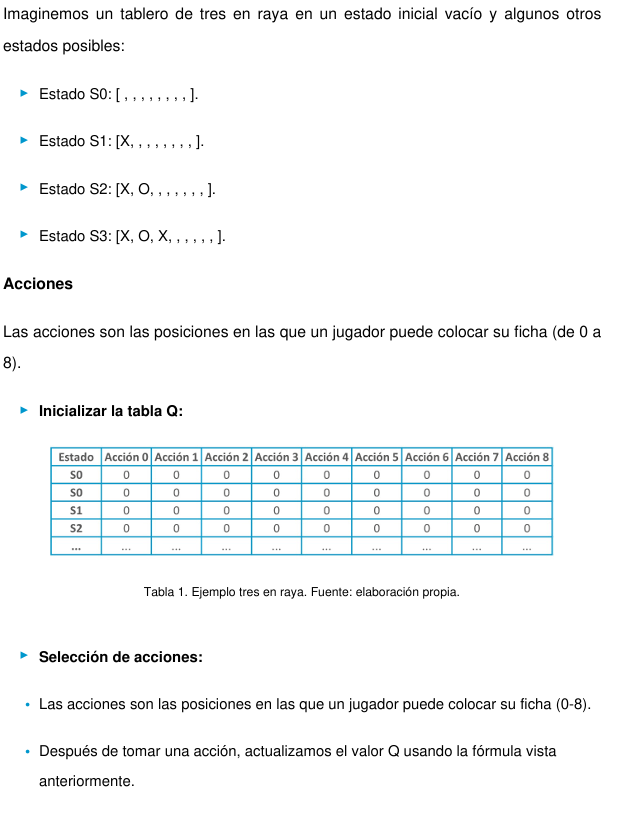
\includegraphics[width=\linewidth]{imagenes/tresenraya1.png}
        \label{fig:tresenraya1}
    \end{minipage}
    \hfill
    \begin{minipage}{0.48\linewidth}
        \centering
        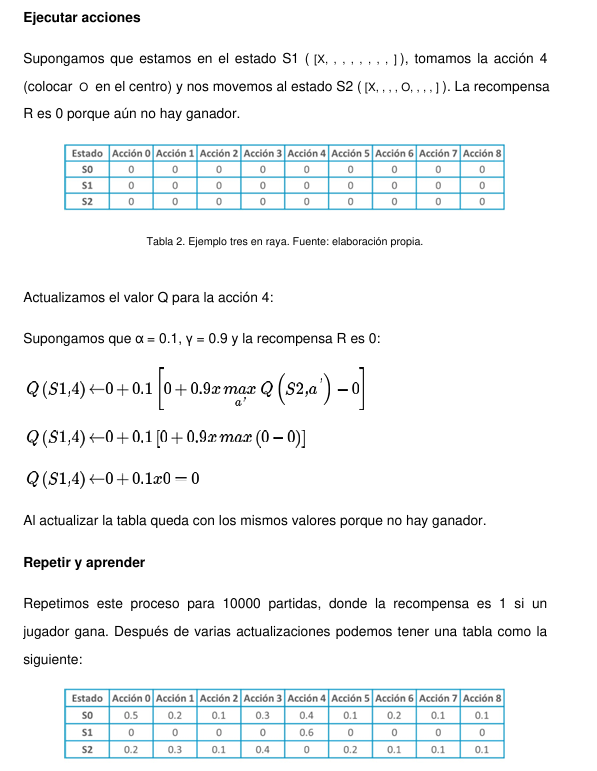
\includegraphics[width=\linewidth]{imagenes/tresenraya2.png}
        \label{fig:tresenraya2}
    \end{minipage}
\end{figure}

\newpage

\section{Deep Q-Network (DQN)}

El algoritmo Q-learning es efectivo en entornos simples, pero resulta inviable cuando el número de estados y acciones crece considerablemente, ya que no es práctico usar una tabla Q. Para superar esta limitación, se desarrolló el \textbf{Deep Q-Network (DQN)}, que combina Q-learning con redes neuronales profundas para aproximar la función Q y manejar grandes espacios de estados.

DQN utiliza dos redes neuronales:
\begin{itemize}
    \item \textbf{Red principal:} parametrizada por $\theta$, estima los valores Q del estado $s$ y acción $a$ actuales, es decir, $Q(s, a; \theta)$.
    \item \textbf{Red objetivo:} parametrizada por $\theta'$, tiene la misma arquitectura que la principal y se utiliza para calcular los valores Q objetivo del siguiente estado $s'$ y acción $a'$. Sus parámetros se actualizan periódicamente copiando los de la red principal.
\end{itemize}

La red Q predice los valores para cada acción y se elige aquella con el valor más alto. El objetivo es minimizar la pérdida del error cuadrático medio (MSE) entre los valores Q predichos y los valores Q objetivo:
\[
Loss = \left(Q_{\text{objetivo}} - Q_{\text{Predicha}}\right)^2
\]

Los valores Q objetivo se calculan usando la ecuación de Bellman:
\[
Q_{\text{target}} = R + \gamma \max(Q_{\text{next}})
\]
donde $R$ es la recompensa obtenida y $Q_{\text{next}}$ es el valor máximo estimado por la red objetivo para el siguiente estado.

Al igual que en Q-learning, la política óptima $\pi$ consiste en seleccionar en cada estado la acción con el mayor valor Q estimado y continuar este proceso para maximizar la recompensa esperada a lo largo del tiempo.

\begin{center}
\begin{tikzpicture}[
  node distance=1.5cm and 2.5cm,
  every node/.style={draw, rounded corners, align=center, minimum width=3.5cm, minimum height=1.2cm, font=\normalsize},
  arrow/.style={-Stealth, thick}
]
\node (estado) {Estado};
\node (redq) [right=of estado] {Red neuronal Q};
\node (valores) [right=of redq, draw=none, align=left, font=\normalsize] {
  Valor Q acción 1\\
  Valor Q acción 2\\
  \vdots\\
  Valor Q acción n
};

\draw[arrow] (estado) -- (redq);
\draw[arrow] (redq) -- (valores);
\end{tikzpicture}
\end{center}





\section{Algoritmo REINFORCE}

El \textbf{algoritmo REINFORCE} (``REward Increment = Nonnegative Factor $\times$ Offset Reinforcement $\times$ Characteristic Eligibility'') es una técnica clásica de aprendizaje por refuerzo basada en el método de gradiente de políticas.

REINFORCE aprende directamente una \textbf{política}: una función que mapea estados a probabilidades de acciones. La política se parametriza (por ejemplo, con una red neuronal) y se ajusta iterativamente mediante el cálculo de gradientes y ascenso de gradiente para maximizar la recompensa acumulada esperada.

El agente interactúa con el entorno siguiendo su política actual, obteniendo una secuencia de recompensas. El retorno acumulado desde el tiempo $t$ se calcula como:
\[
R_t = r_t + \gamma r_{t+1} + \gamma^2 r_{t+2} + \cdots + \gamma^{T-t-1} r_{T-1}
\]
donde $r_t$ es la recompensa en el paso $t$, $\gamma$ es el factor de descuento y $T$ es el último paso del episodio.

El gradiente para actualizar los parámetros de la política es:
\[
\Delta\theta = \alpha \nabla_\theta \log \pi_\theta(a_t|s_t) R_t
\]
donde $\alpha$ es la tasa de aprendizaje, $\nabla_\theta \log \pi_\theta(a_t|s_t)$ es el gradiente logarítmico de la política y $R_t$ la recompensa acumulada.

\subsection*{Conceptos clave}
\begin{itemize}
    \item \textbf{Política ($\pi$):} Estrategia que sigue el agente para tomar decisiones, parametrizada como $\pi^\theta(a|s)$.
    \item \textbf{Función de recompensa acumulada ($R$):} Suma de recompensas recibidas a lo largo de un episodio.
    \item \textbf{Gradiente de la política:} Se utiliza para ajustar los parámetros de la política en la dirección que maximiza la recompensa esperada.
\end{itemize}


\section{Proximal Policy Optimization (PPO)}

OpenAI publicó un artículo denominado \textit{Algoritmos de optimización de políticas próximas} (PPO) como una nueva familia de métodos de gradiente de políticas. PPO es conocido por ser robusto y eficiente, y se utiliza para entrenar agentes en entornos donde las decisiones se toman en base a políticas, es decir, reglas que determinan las acciones a tomar en cada estado del entorno.

\subsection{Tres puntos principales}
\begin{itemize}
    \item \textbf{PPO alterna} entre el muestreo de datos a través de la interacción con el entorno y la optimización de una función objetivo-sustituta mediante un ascenso de gradiente estocástico.
    \item A diferencia de los métodos de gradiente de políticas estándar, que realizan una actualización de gradiente por muestra de datos, PPO introduce una función objetivo novedosa que permite múltiples épocas de actualizaciones en minibatch.
    \item PPO ofrece algunos de los beneficios de la optimización de políticas de región confiable (TRPO), pero es más simple de implementar, más general y tiene una mejor complejidad de muestra empíricamente.
\end{itemize}

\subsection{Conceptos clave en este algoritmo}
\begin{itemize}
    \item \textbf{Función de valor} ($V$): mide lo bueno que es estar en un estado en particular.
    \item \textbf{Ratio de probabilidad} ($r_t(\theta)$): es el ratio entre la nueva política y la política antigua. Es clave en PPO para medir el cambio de la política:
    \[
    r_t(\theta) = \frac{\pi_\theta(a_t|s_t)}{\pi_{\text{old}}(a_t|s_t)}
    \]
    \item \textbf{Clip objetivo}: se introduce una función objetivo que limita (clip) los ratios de probabilidad para mantener actualizaciones de política dentro de un rango razonable.
\end{itemize}

La función objetivo es:
\[
L^{\text{CLIP}}(\theta) = \mathbb{E}_t \left[ \min \left( r_t(\theta) \hat{A}_t, \; \text{clip}\left(r_t(\theta), 1 - \epsilon, 1 + \epsilon \right)\hat{A}_t \right) \right]
\]
donde $\hat{A}_t$ es la ventaja estimada y $\epsilon$ es un hiperparámetro que controla cuánto puede cambiar el ratio de probabilidad.

\subsection{Entrenamiento del algoritmo PPO}
El algoritmo PPO se entrena de la siguiente manera:
\begin{enumerate}
    \item Recolección de datos, ejecutando la política actual para recolectar datos de interacción del agente con el entorno.
    \item Estimación de la ventaja $\hat{A}_t$ para cada acción tomada.
    \item Actualización de la política utilizando $L^{\text{CLIP}}(\theta)$ para asegurar que las actualizaciones no sean demasiado grandes.
    \item Este proceso se repite, ajustando la política gradualmente para mejorar el desempeño del agente.
\end{enumerate}





\section{Comparativa de técnicas aprendizaje por refuerzo}


\begin{figure}[ht]
    \centering
    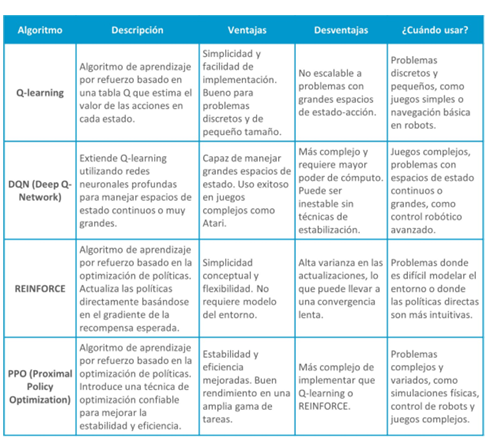
\includegraphics[width=1\linewidth]{imagenes/comparativa-q-learning.png}
    \label{fig:comparativa-q-learning}
\end{figure}


\end{document}
